\chapter{Results and discussion\label{sec:Results}} \markright{\thechapter~Results and analysis}

This chapter presents the results of the residential and office case studies. For each case, the governing design criteria are first analysed, followed by the best cross-sections for a representative span every compared floor system. Then the systems are compared to each other across the sustainability assessment criteria.

\section{Residential case}
\subsection{Analysis of slab systems} 
\begin{figure}[htbp]
    \centering
    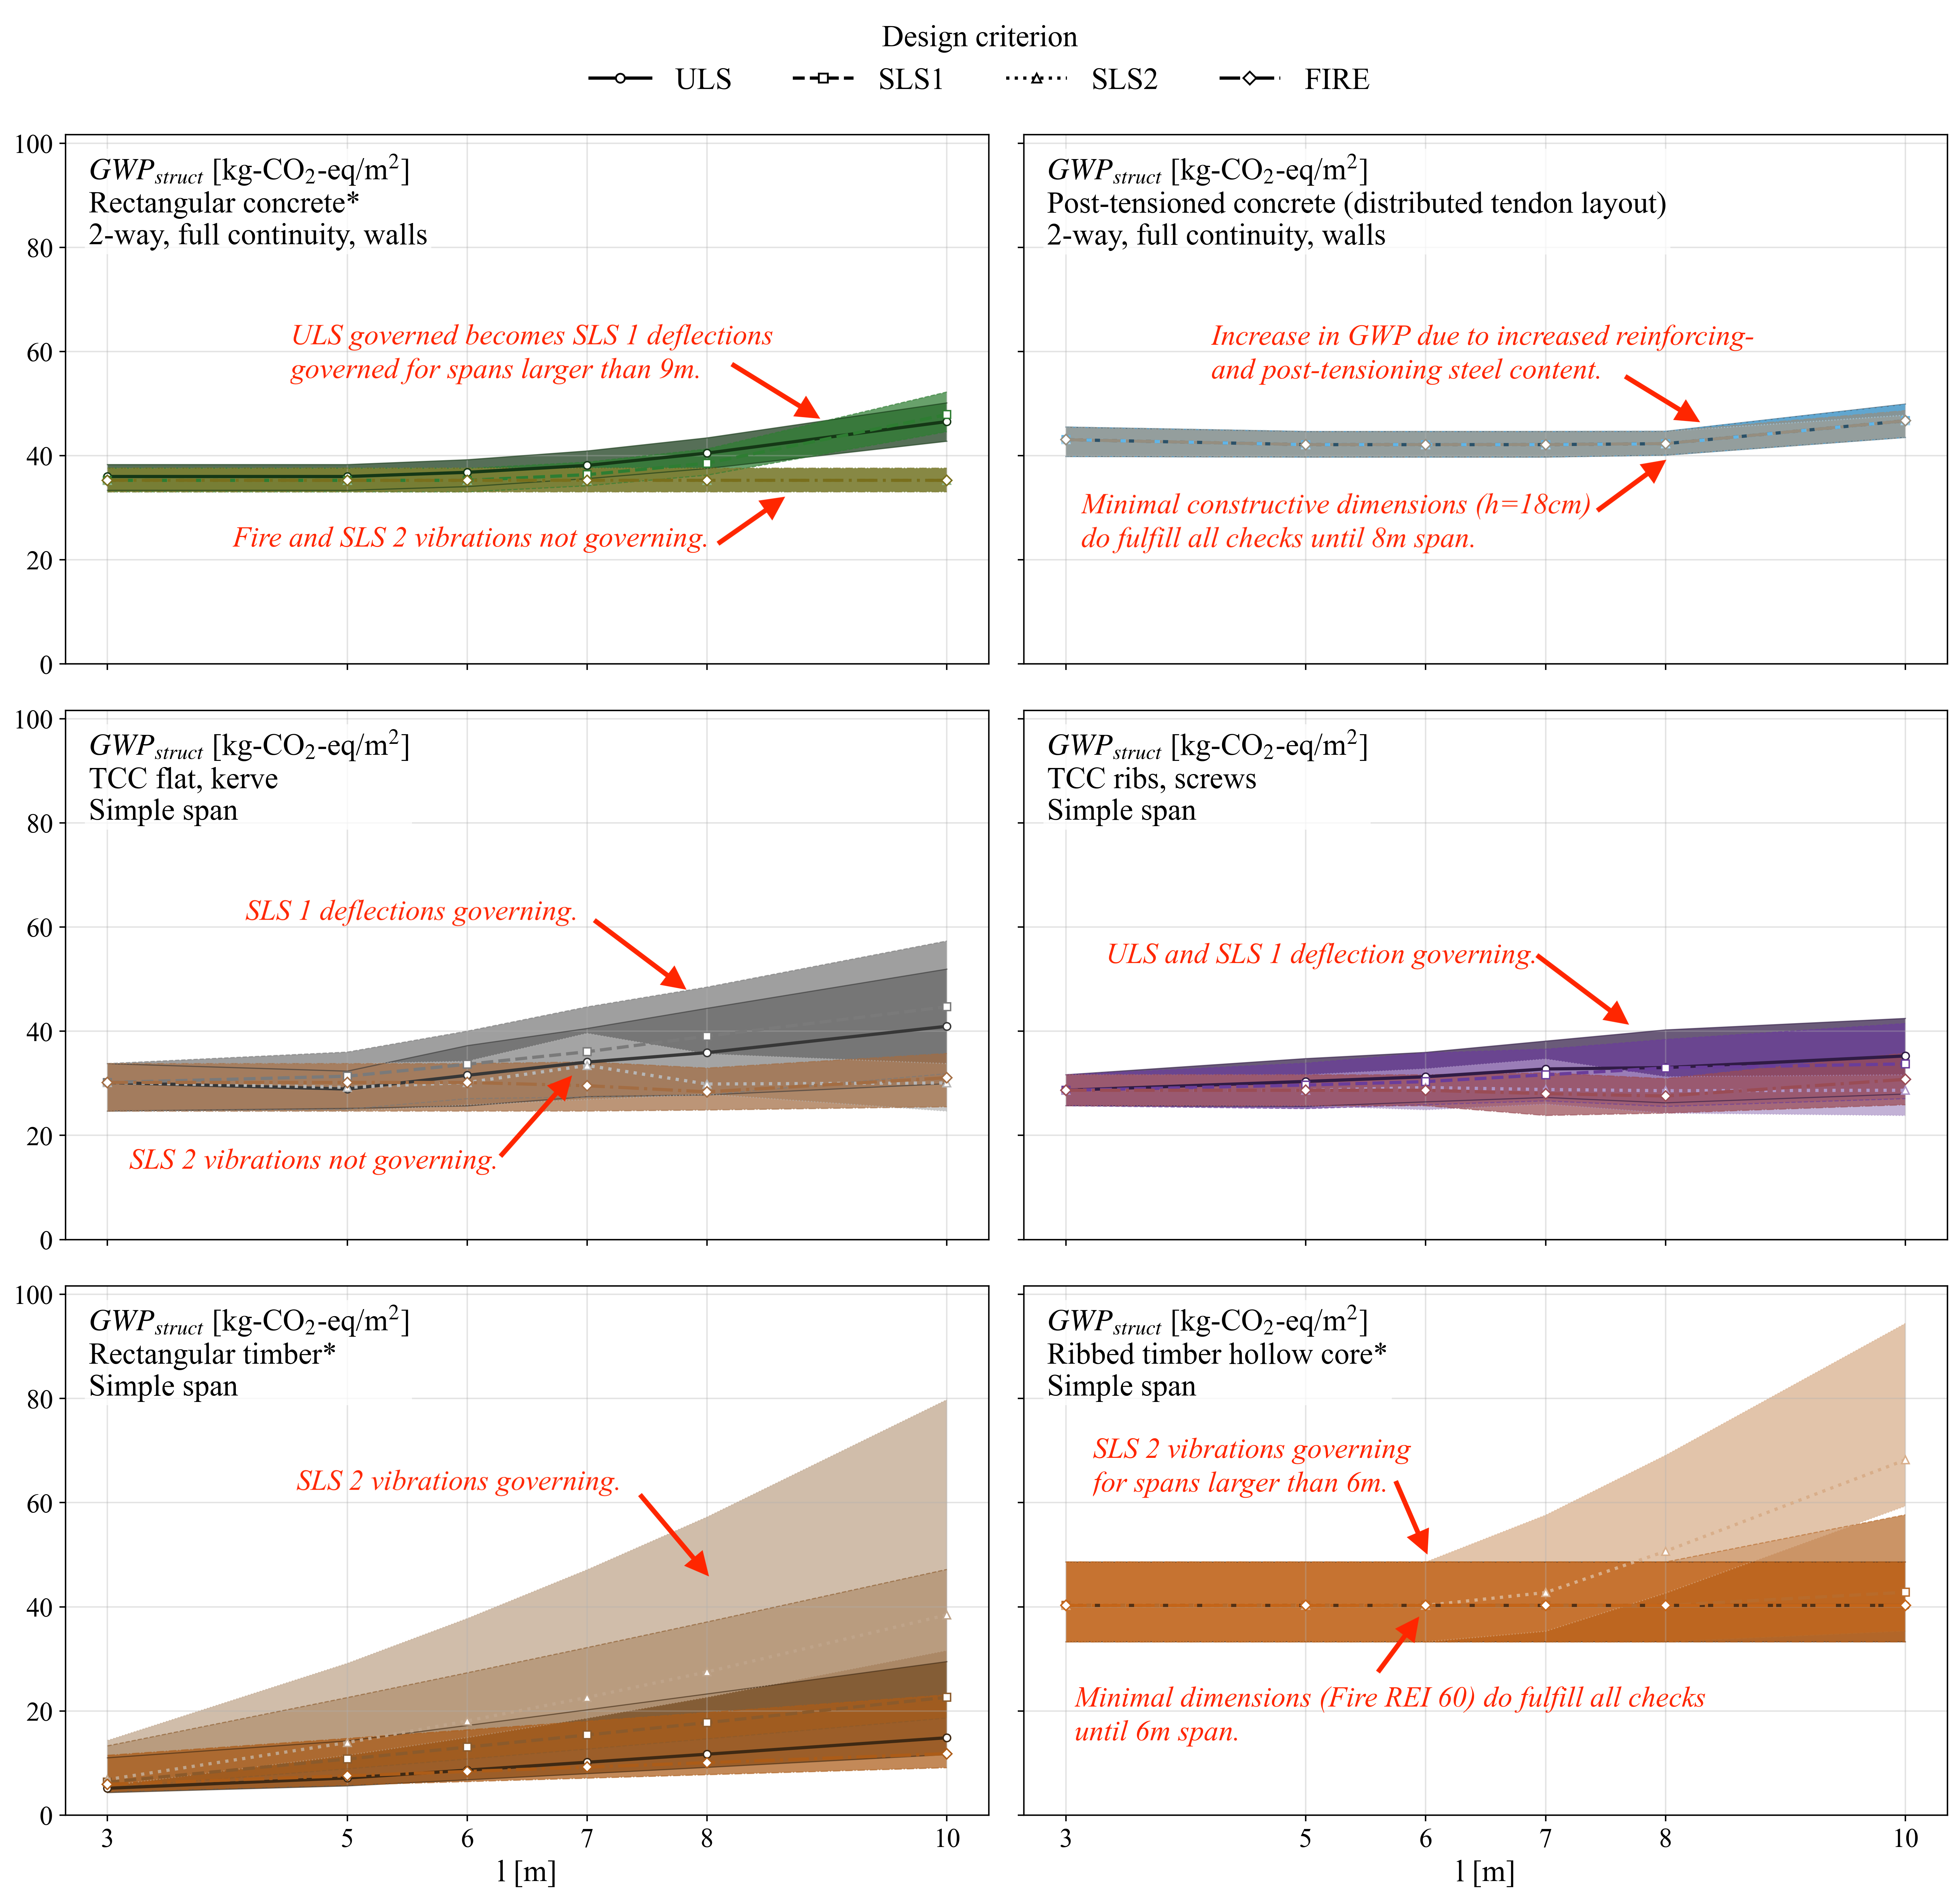
\includegraphics[width=1\textwidth]{IMAGES/final_single_residential_GWP_struct.png}
    \caption{GWP required to fulfil each respective design criterion of the structural cross-section for the residential case.}
    \label{fig:final_single_residential_GWP_struct}
\end{figure}

Figure~\ref{fig:final_single_residential_GWP_struct} shows the $GWP_{\mathrm{struct}}$ required by each system to fulfil the respective design criterion for the residential case. The values refer to the structural cross-section only, while the additional load of the floor build-up is already included in the structural model.

For the rectangular reinforced concrete slab, the governing criteria are ULS and SLS~1 deflection. Vibration and fire requirements are already fulfilled by the minimum dimensions and therefore do not lead to an increase over the investigated span range. SLS~1 deflection becomes governing only for spans larger than approximately $9,\mathrm{m}$. In engineering practice, deflection is often expected to govern the design \cite{Kaufmann2024_WhitePaper}. However, the present model set-up uses a favourable static system, with a rectangular layout, wall supports, two-way load transfer, and full continuity, which improves the deflection behaviour.

For the post-tensioned concrete slab, the results are governed by minimum detailing dimensions up to a span of approximately $8,\mathrm{m}$. For larger spans, $GWP_{\mathrm{struct}}$ increases due to the higher reinforcement and post-tensioning steel content required to satisfy the ULS design state. Compared with the conventionally reinforced concrete slab, SLS~1 deflection does not become governing. This confirms the intended serviceability improvement achieved through post-tensioning \cite{Rombach2010}.

\newpage
For the rectangular timber slab, SLS~2 vibration requirements govern over the investigated span range. Consequently, the available reserves in ULS, fire, and SLS~1 deflection cannot be exploited. For the ribbed timber hollow-core system, the minimum dimensions required to fulfil the REI~60 fire requirement govern up to a span of approximately $6,\mathrm{m}$. Beyond this span, SLS~2 vibration requirements also become governing. It can therefore be concluded that the dimensions of timber sections need to be increased primarily to satisfy vibration criteria.

For the timber--concrete composite systems, the SLS~2 vibration criterion does not become governing. This supports the improved vibration behaviour of TCC systems reported in the literature \cite{proHolz2012_Zuschnitt45}. Instead, the governing criteria are ULS and SLS~1 deflection.

Overall, cross-sections containing concrete show a smaller variation in $GWP_{\mathrm{struct}}$ across the design states. This supports that concrete contributes to the functional performance of floor systems, since its stiffness, mass and fire resistance can help satisfy several design requirements simultaneously. These functional advantages also help explain the continued prevalence of concrete floor systems in practice \cite{Priore2024_CarbonImpactSlabs, Ammann2024}.

\newpage
\subsection{Best cross-section}
Figure~\ref{fig:final_cross_sections_residential_6m} shows the best \(GWP_{tot}\) cross-sections for the residential case at a span of \(6\,\mathrm{m}\). The breakdown of GWP, cost and construction time underlines the importance of assessing the complete floor system rather than the structural cross-section alone. Across all residential systems, the acoustic floor build-up contributes a substantial share of \(GWP_{tot}\), construction cost, and construction time. 

\begin{figure}[H]
    \centering
    
\includegraphics[width=1\textwidth]{IMAGES/final_cross_sections_residential_6m.png}
    \caption{Best \(GWP_{tot}\) cross-sections for the residential case at a span of \(6\,\mathrm{m}\).}
    \label{fig:final_cross_sections_residential_6m}
\end{figure}


\subsection{Comparison of residential floor systems}
Figure~\ref{fig:final_env_comparison_residential} compares the residential floor systems over the investigated span range and illustrates the variation resulting from the considered material and product datasets. 
\begin{figure}[H]
    \centering
    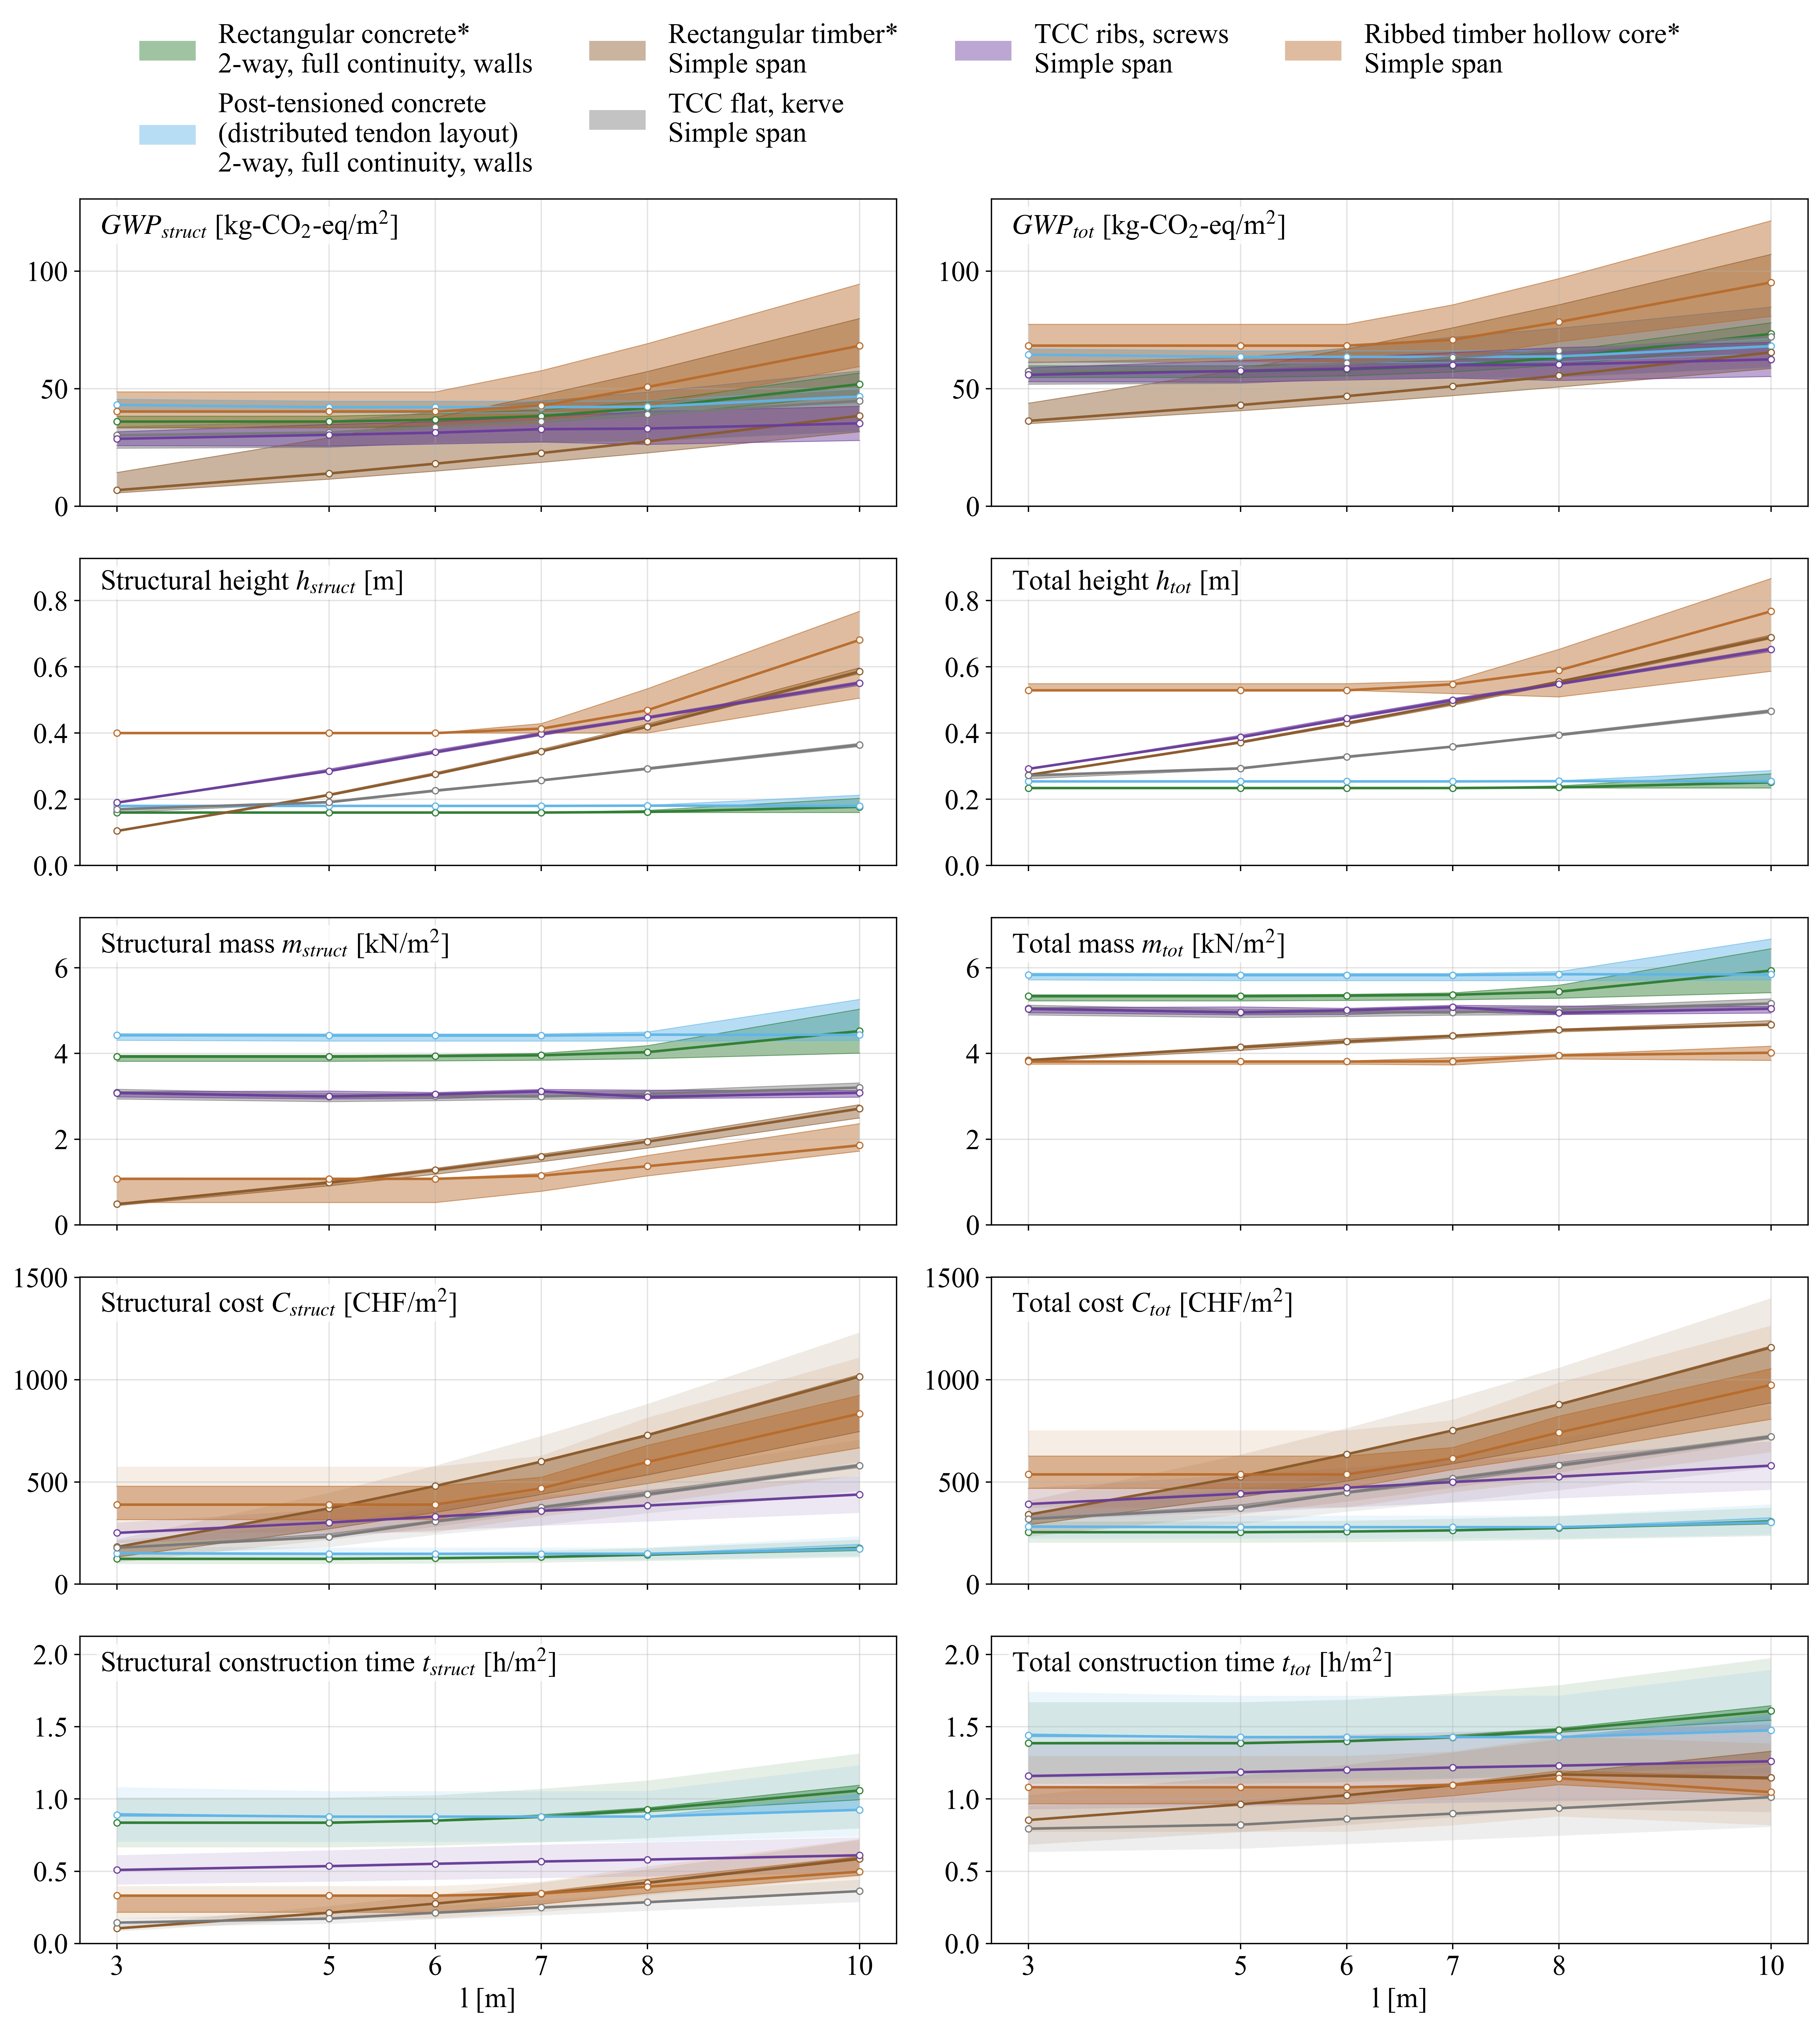
\includegraphics[width=1\textwidth]{IMAGES/final_env_comparison_residential.png}
    \caption{Comparison according to sustainability assessment criteria of selected floor systems for residential buildings.}
    \label{fig:final_env_comparison_residential}
\end{figure} 

Figure~\ref{fig:uq_pairwise_scores_Residential} complements this comparison by a pairwise comparison that accounts for overlaps between the resulting performance ranges. A pairwise score of \(0.8\) indicates that the respective system has an average probability of \(80\,\%\) of outperforming the systems positioned below it in the figure.
\begin{figure}[H]
    \centering
    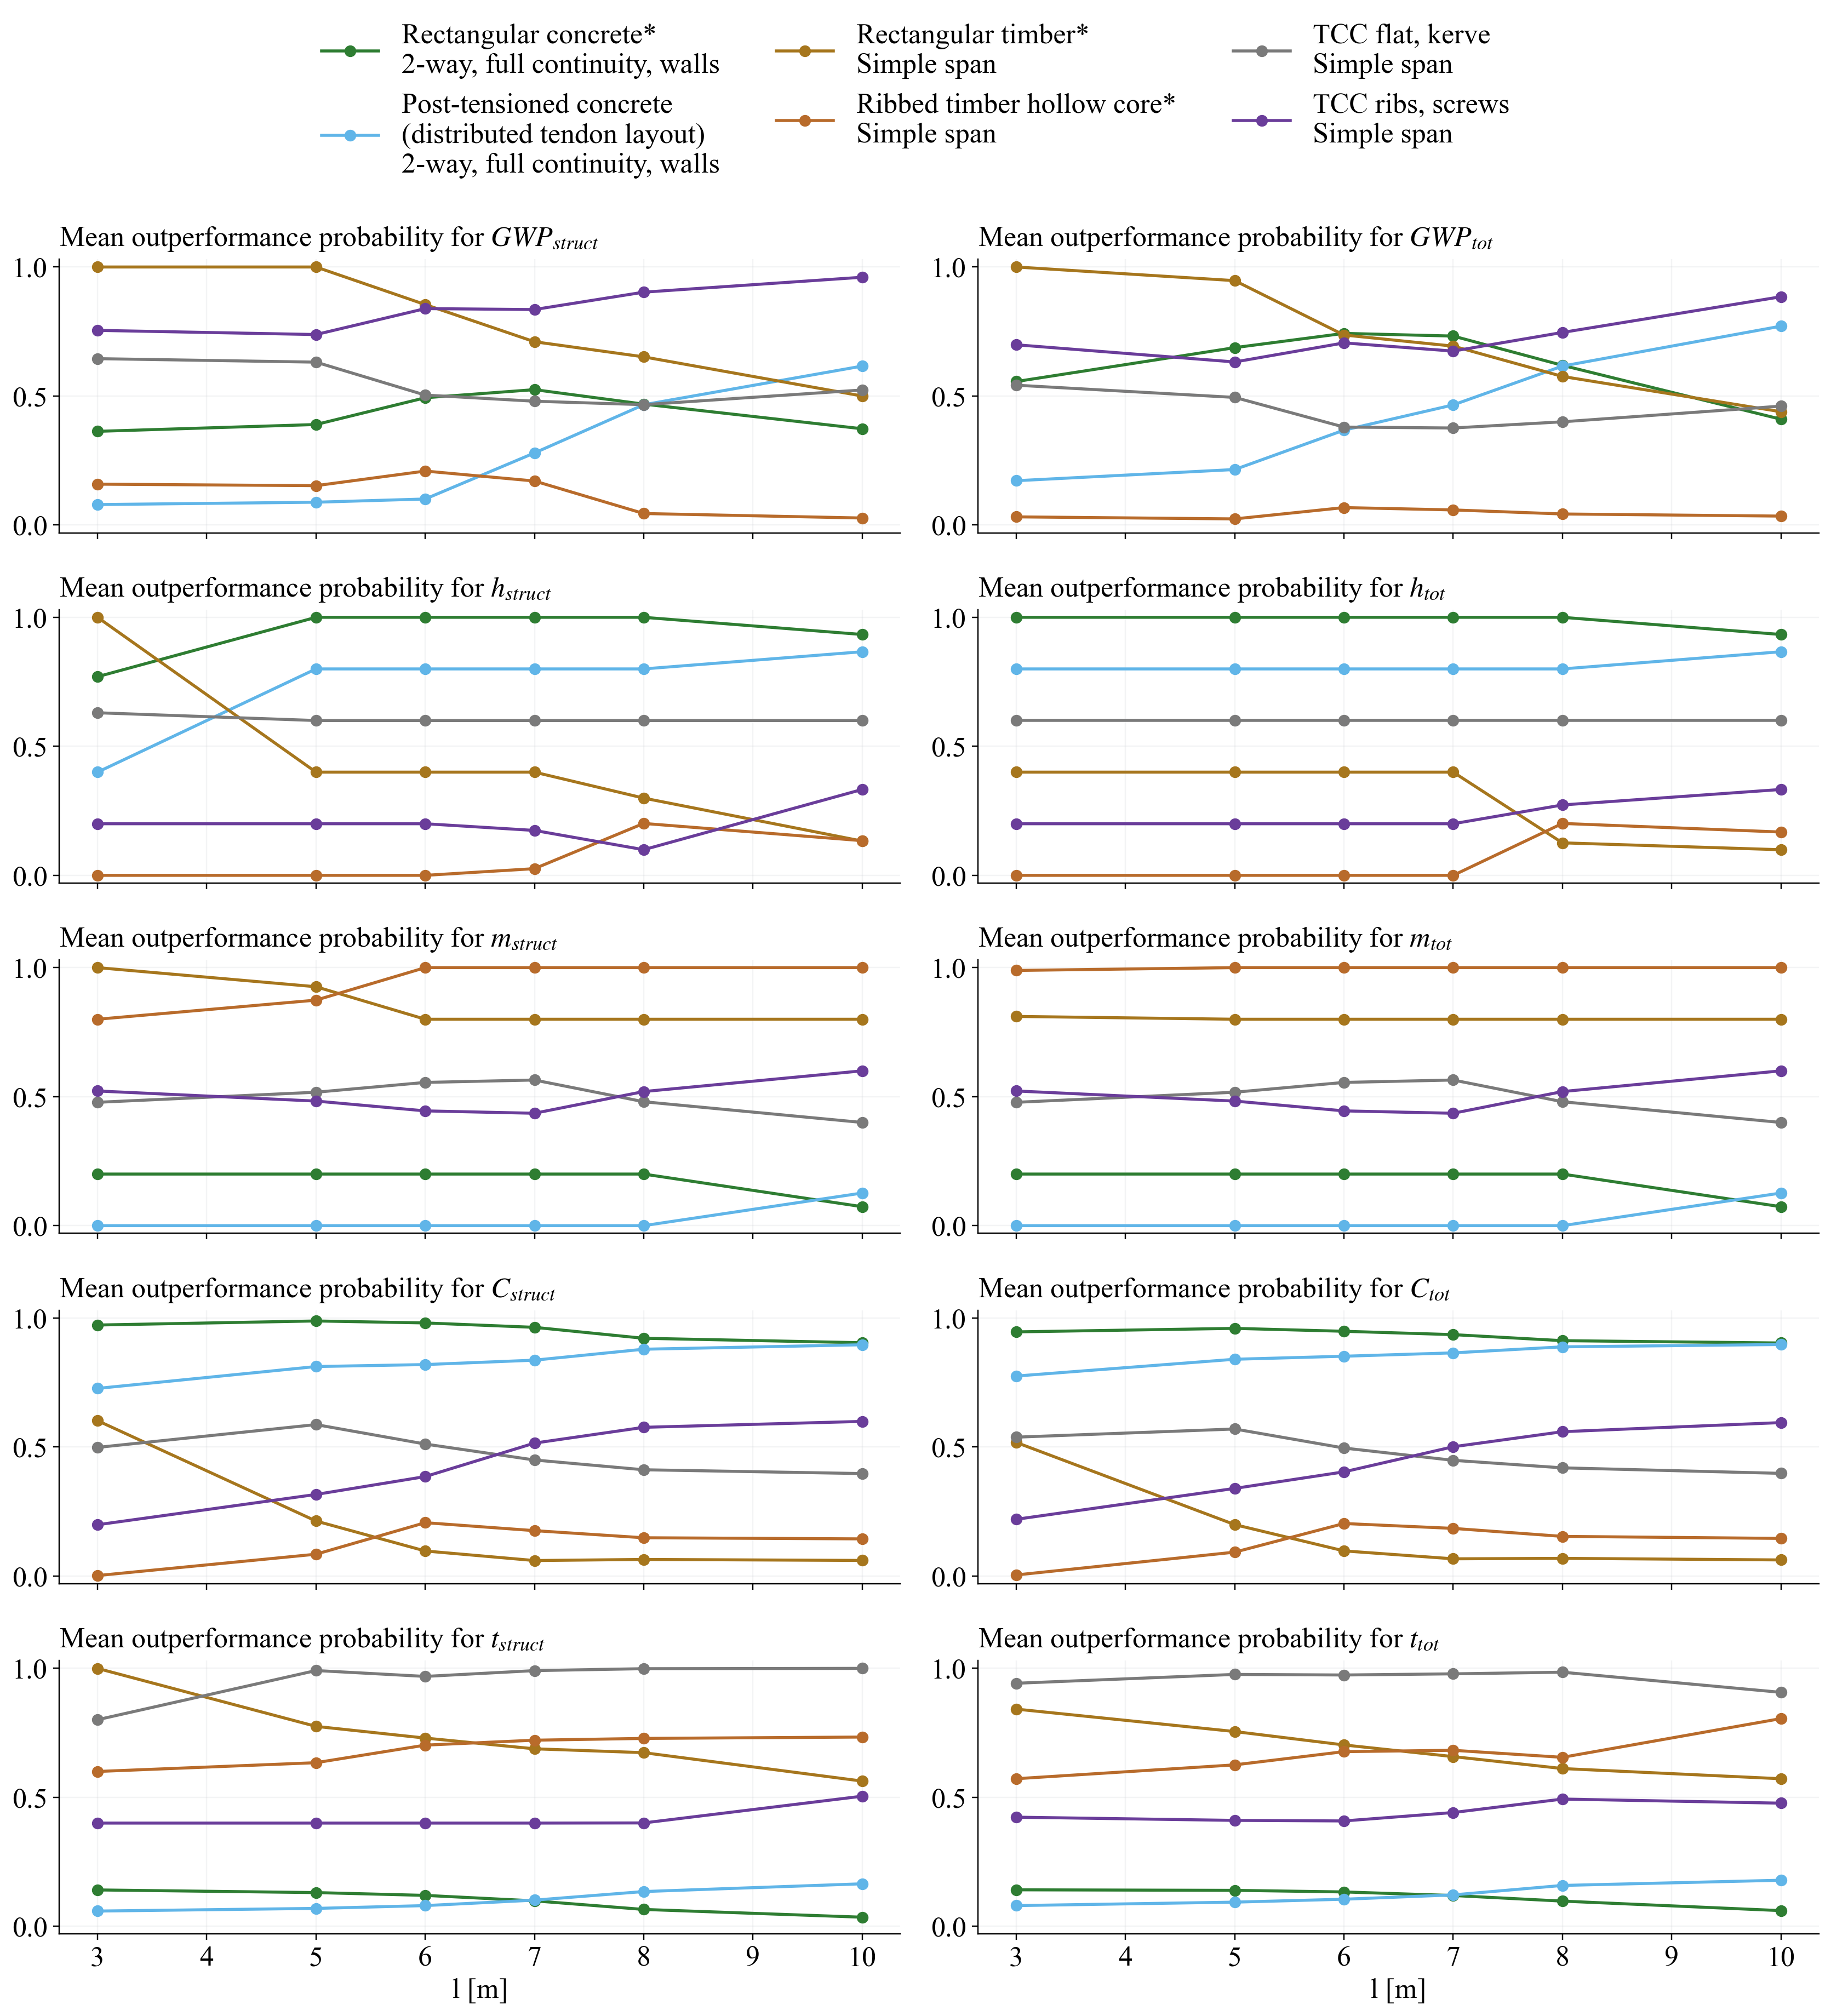
\includegraphics[width=1\textwidth]{IMAGES/uq_pairwise_scores_Residential.png}
    \caption{Pairwise comparison according to sustainability assessment criteria of selected floor systems for residential buildings.}
    \label{fig:uq_pairwise_scores_Residential}
\end{figure}

\newpage
Both figures distinguish between the structural cross-section and the total floor system, with the latter additionally accounting for the acoustic floor build-up. This distinction is particularly important for timber and timber--concrete composite systems, whose acoustic build-ups are generally heavier, deeper, and more emission-intensive than those of concrete systems. This observation is consistent with the multilayer timber floor configurations documented by Lignum \cite{LignumData_Decken}.


\subsubsection{Global warming potential}

Rectangular timber achieves the lowest structural GWP for spans between \(3\) and \(5\,\mathrm{m}\). For larger spans, its vibration behaviour increases the required dimensions notably, resulting in the strongest increase in GWP over the span.
At intermediate spans of approximately \(6\) to \(7\,\mathrm{m}\), rectangular reinforced concrete becomes the best-performing system. Here, reinforced concrete uses its highly efficient two-way structural system with full continuity. Above approximately \(7\,\mathrm{m}\), ribbed TCC and post-tensioned concrete become increasingly competitive. This is consistent with the span range in which post-tensioning is generally considered structurally effective \cite{Rombach2010}.

Ribbed TCC achieves particularly low structural GWP at longer spans because its structurally efficient ribbed cross-section reduces material consumption. This advantage comes at the cost of a substantially increased construction depth. Flat TCC exhibits slightly higher structural GWP, with the difference between the two TCC systems increasing with span.

The pairwise comparison modifies the interpretation of these span limits. When all total-system criteria are considered together, rectangular timber is only the clear overall winner at \(3\,\mathrm{m}\). Flat TCC obtains the highest total pairwise score at \(5\,\mathrm{m}\) and again at \(8\,\mathrm{m}\), mainly because it combines competitive GWP with moderate height and short construction time. Rectangular reinforced concrete narrowly leads the total pairwise comparison at \(6\) and \(7\,\mathrm{m}\), where its low cost and low construction height compensate for its higher GWP. At \(10\,\mathrm{m}\), ribbed TCC becomes the highest-ranked system, although post-tensioned concrete and flat TCC remain close alternatives. The span recommendations should therefore be understood as robust multi-criteria ranges rather than as direct transitions between the lowest deterministic \(GWP_{tot}\) values.

The ribbed timber hollow-core system exhibits the highest structural GWP across most of the investigated span range. At shorter spans, this can be explained by the governing minimum dimensions required by the simplified fire-design model. A more refined fire verification could reveal further potential. In addition, the result is strongly influenced by the assumed hollow-core insulation. It must therefore be interpreted cautiously, as alternative insulation products could substantially affect the environmental performance.

\subsubsection{Height}
The slender rectangular concrete achieves the lowest total floor height until a span of \(8\,\mathrm{m}\). The post-tensioned concrete is limited by its geometrical minimum dimensions due to detailing of the anchorage and post-tensioning tendons. However, it surpasses the rectangular concrete cross-section for spans larger than \(8\,\mathrm{m}\).

Rectangular timber remains competitive up to approximately \(5\,\mathrm{m}\) and acceptable between \(5\) and \(7\,\mathrm{m}\), but its required depth increases substantially at longer spans. Flat TCC achieves a lower total height than the pure timber systems and ribbed TCC. Ribbed TCC provides high material efficiency but requires a considerably greater structural depth, particularly at longer spans.

The results also demonstrate the relevance of floor height as a sustainability assessment criterion. According to the Building and Zoning Regulations of the City of Zurich, the permissible building height in zone W5 is generally limited to \(18\,\mathrm{m}\) \cite{StadtZuerich_Bauordnung_700100}. Assuming a clear room height of \(2.4\,\mathrm{m}\), six storeys are possible only if the total floor depth remains below \(0.6\,\mathrm{m}\). Floor height can therefore directly affect the achievable service area. This is critical when trying to achieve a high service area in relation to the total invested carbon of the building \cite{Kaufmann2024_WhitePaper}. For the investigated example, imposing \(h_{\mathrm{tot}}\leq 0.6\,\mathrm{m}\) would exclude rectangular timber, ribbed timber hollow-core, and ribbed TCC solutions at spans above approximately \(7\,\mathrm{m}\), showing the importance of this sustainability assessment criterion.

\subsubsection{Mass}
At the structural level, the timber-based systems are substantially lighter than the concrete systems. However, this difference decreases when the complete floor system is considered because the timber and TCC systems require relatively heavy acoustic floor build-ups. Consequently, the total mass of the investigated systems generally lies between approximately \(400\) and \(600\,\mathrm{kg/m^2}\), which is consistent with floor configurations documented by Lignum \cite{Lignum2021_HBT1}.

Thus, for buildings founded on soil with sufficient bearing capacity, differences in floor mass are unlikely to cause major changes in the environmental impact of the substructure. The relevance of mass may increase under poor ground conditions.

Additionally, mass also affects seismic actions. However, this benefit cannot be evaluated independently of the height. Here, the lightweight systems require greater floor depths, potentially increasing the total building height and altering the seismic response. A conclusive building-level assessment therefore requires the combined consideration of floor mass and structural height. 

Most importantly, the magnitude of the indirect influences on the foundation and the lateral load-resisting structural system depends on the number of storeys. For a conventional residential building with fewer than six storeys, mass is therefore proposed to be handled as a secondary sustainability assessment criterion.

\subsubsection{Construction cost}
Rectangular concrete achieves the lowest construction cost until spans of \(9\,\mathrm{m}\). This reflects both the economic efficiency of established concrete construction processes and the low material price of concrete. It must be noted that post-tensioned concrete is economically competitive across all spans and even surpasses traditional reinforced concrete above spans of \(9\,\mathrm{m}\). This is attributed to the reduced total steel content of the post-tensioned concrete.

The timber systems are among the most expensive alternatives. This result should be interpreted cautiously because their unit price is defined per cubic metre and implicitly accounts for connections and fabrication. In practice, the relative contribution of these components may decrease as member dimensions increase. The present model may therefore overestimate the cost of large timber cross-sections.

Ribbed TCC is more expensive than flat TCC up to approximately \(7\,\mathrm{m}\). This is primarily caused by the screw connectors, each of which is explicitly included in the cost model. At longer spans, the material efficiency of the ribbed system becomes more influential.

Post-tensioned concrete becomes economically competitive with conventional reinforced concrete at approximately \(8\,\mathrm{m}\) and above. At these spans, its lower material demand increasingly compensates for the additional post-tensioning components.

\subsubsection{Construction time}
Flat TCC exhibits a comparatively short construction time. The timber component serves as permanent formwork, while the notched connectors can be prefabricated before installation \cite{Morkoetter2021_HBVDecken}.

Ribbed TCC requires more construction time than flat TCC at shorter and intermediate spans because of the larger number of individually installed screw connectors \cite{Morkoetter2021_HBVDecken, Wuerth2021_HolzBetonVerbund}.

Rectangular timber also performs favourably regarding construction time, even outperforming the flat TCC cross-section at a span of \(3\,\mathrm{m}\). The steep increase in construction time for the timber cross-section is, however, an indication that assuming cost and construction time to depend only on the volume used for timber cross-sections is not adequate. For more precise modelling, it is proposed to assume a fixed installation cost and construction time, accompanied by a value per volume to account for higher material usage.

Post-tensioned concrete outperforms conventional reinforced concrete at spans above \(7\,\mathrm{m}\). The additional effort required for tendon installation is increasingly offset by the reduced cross-sectional dimensions and material quantities. The model does not account for the reduced propping time enabled by post-tensioning. Due to the compensation of permanent loads, the formwork can be removed earlier, additionally improving construction progress and making the overall project economically more competitive.



\section{Office case}
\subsection{Analysis of slab systems} 
Figure~\ref{fig:final_single_office_GWP_struct} shows all systems of the office case and compares the required \(GWP_{struct}\) needed to fulfil the respective design criteria. Since only concrete systems are considered, neither the SLS~2 vibration criterion nor the fire criterion becomes governing. 

\begin{figure}[H]
    \centering
    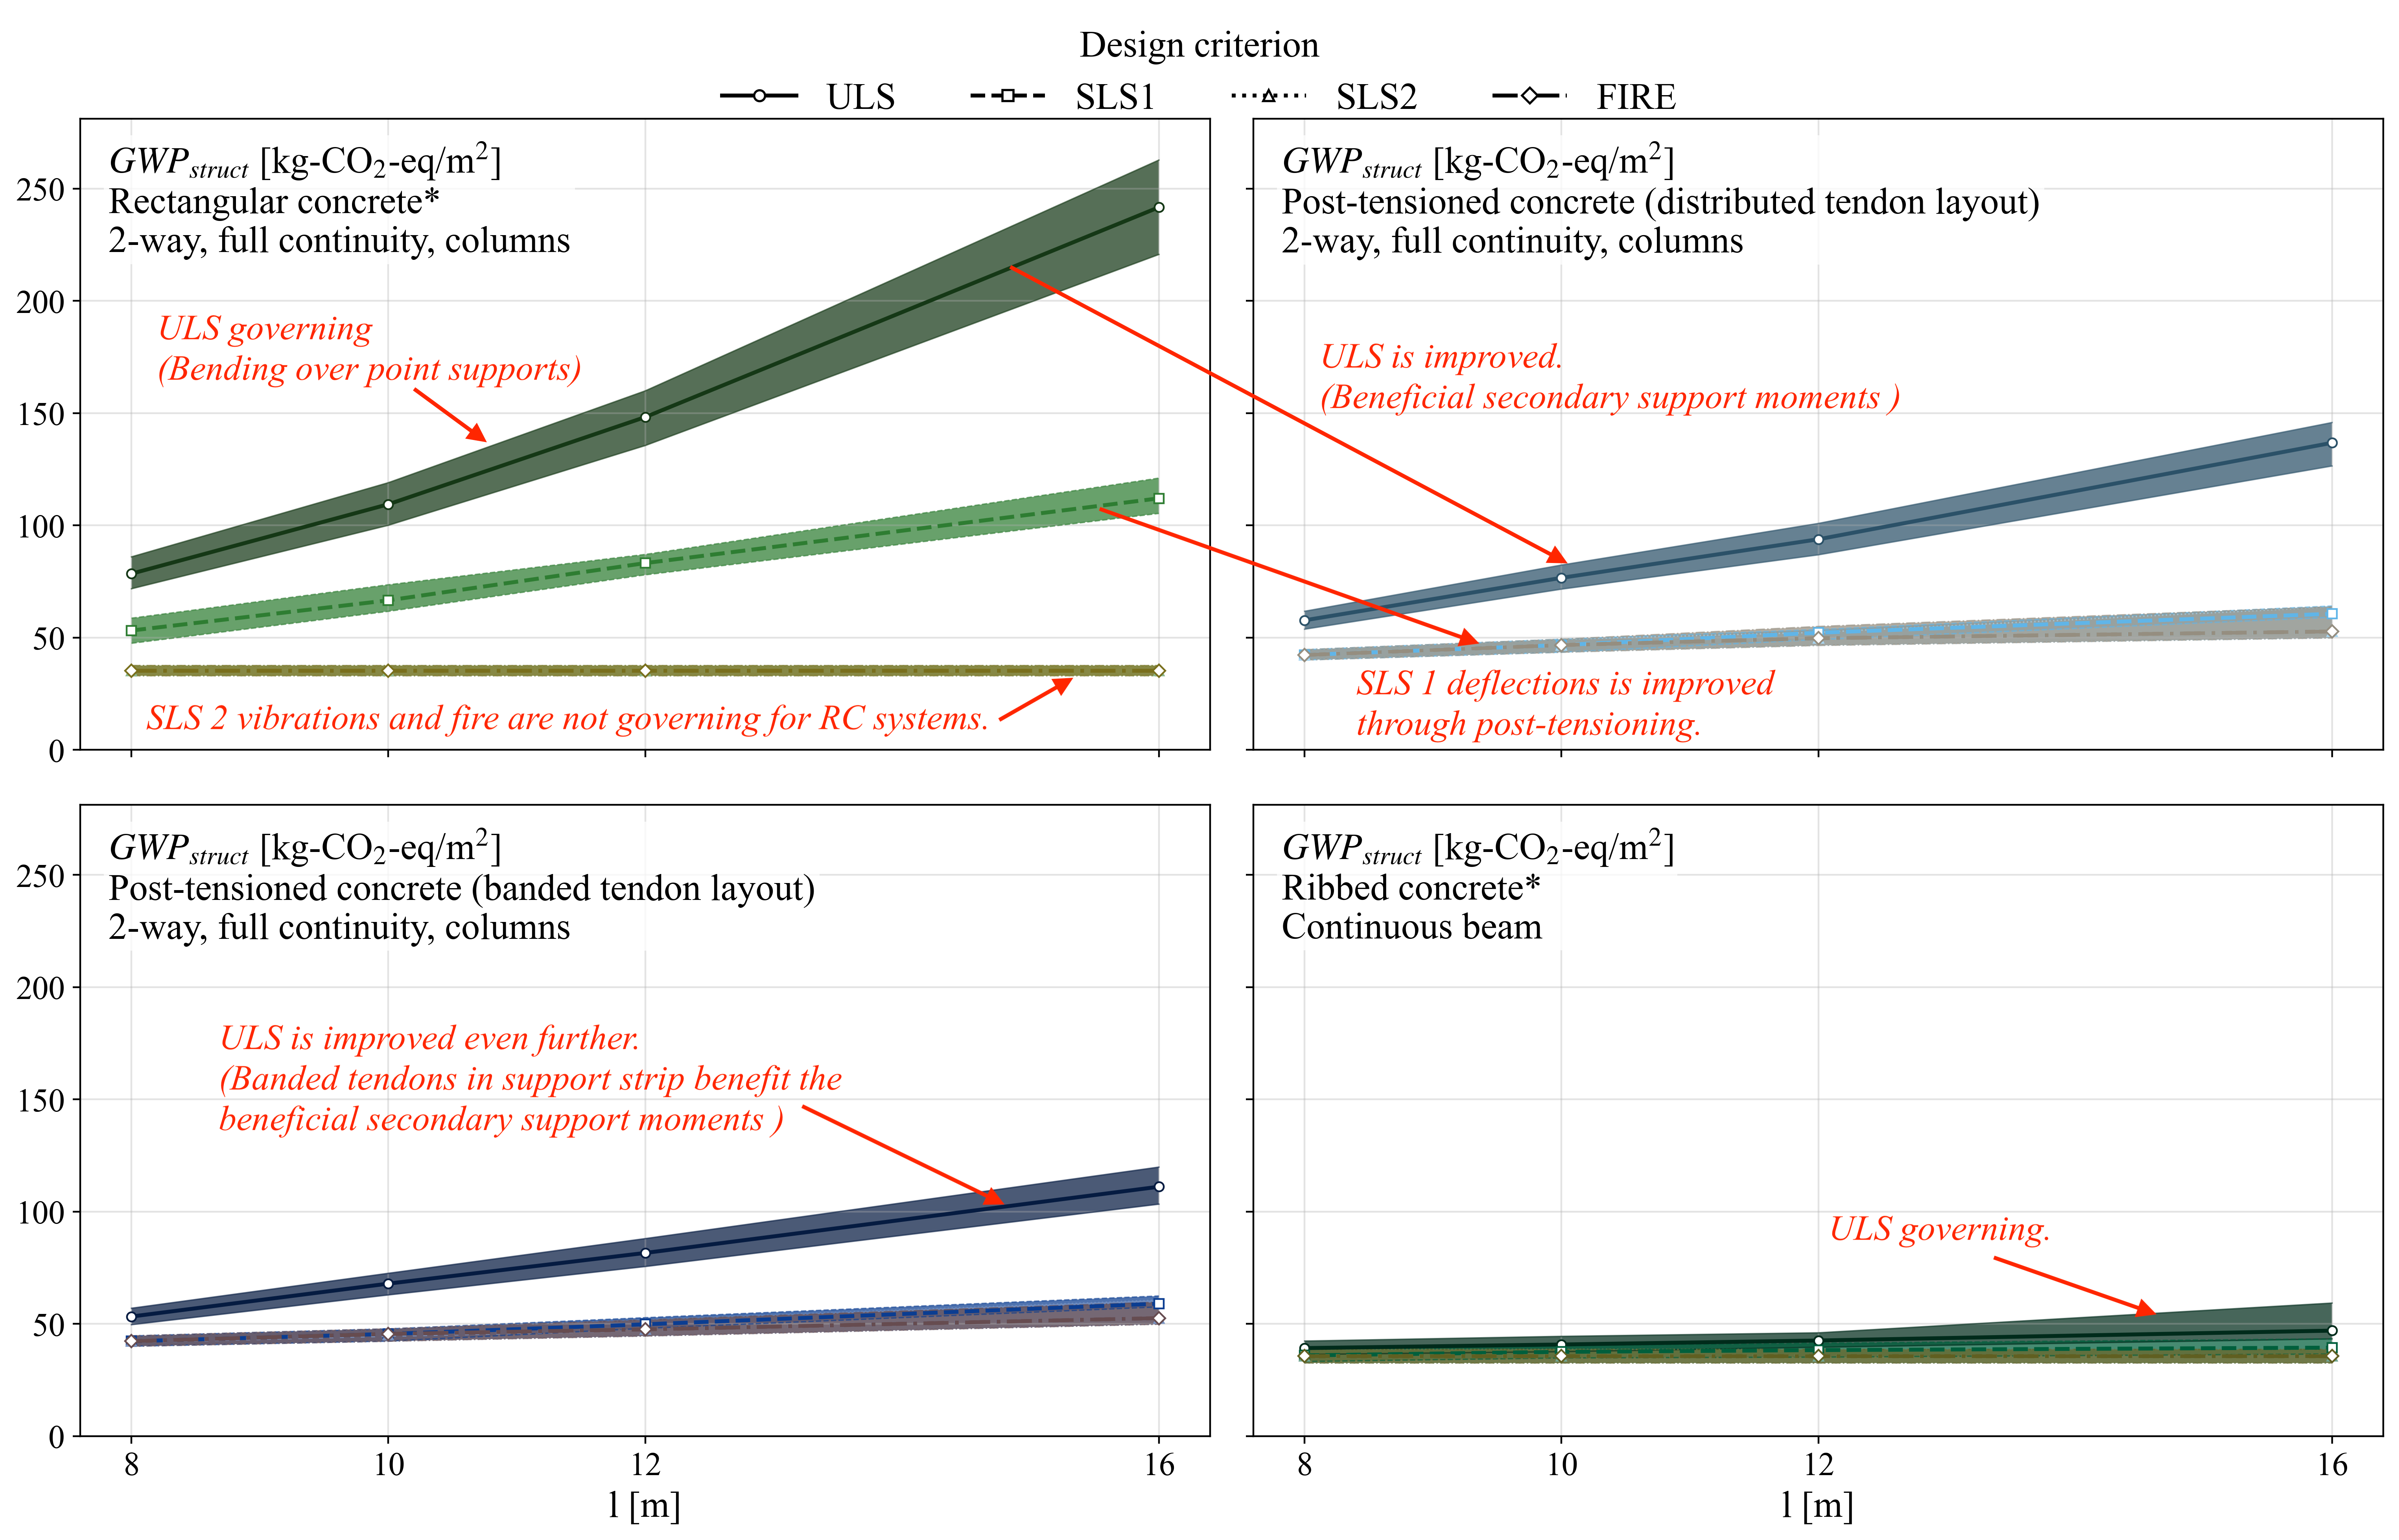
\includegraphics[width=1\textwidth]{IMAGES/final_single_office_GWP_struct.png}
    \caption{GWP required to fulfil each respective design criterion of the structural cross-section for the office case.}
    \label{fig:final_single_office_GWP_struct}
\end{figure}


\newpage
For the point-supported systems, namely the rectangular reinforced concrete and solid post-tensioned concrete slabs, ULS is governed by the negative bending moments over the supports. In the post-tensioned systems, the ULS demand is reduced by beneficial secondary moments generated above the columns. This effect is more pronounced for the banded tendon layout, as the tendons are concentrated within the column strips, where the governing ULS verifications are performed in the present model.
Additionally, the improved punching behaviour of post-tensioned slabs reduces the required amount of punching reinforcement, thereby lowering the GWP compared to conventionally reinforced slabs. Here, the banded layout also performs better, as the deviation forces of all tendons are assumed to counteract the punching load.

The comparison also shows that SLS~1 deflection requirements are improved when moving from conventional reinforced concrete to post-tensioned concrete. This is relevant because deflections may become critical at larger spans, particularly when serviceability limits are not only defined relative to the span, but also by absolute deformation limits. Such absolute limits can be important when non-structural elements, such as interior walls or finishes, cannot accommodate the resulting deflections for the longer compared office spans.

Ribbed concrete is also governed by ULS. However, the different design criteria lie comparatively close to each other, indicating that the system is structurally highly optimised. 

\newpage
\subsection{Best cross-section}
Figure~\ref{fig:final_cross_sections_office_12m} shows the best \(GWP_{tot}\) cross-sections for the office case at a span of \(12\,\mathrm{m}\). The reduced punching reinforcement demand of the post-tensioned systems is validated by their lower required punching shear reinforcement resistance \(V_{Rd,s}\) compared with the conventionally reinforced concrete slab.

\begin{figure}[H]
    \centering
    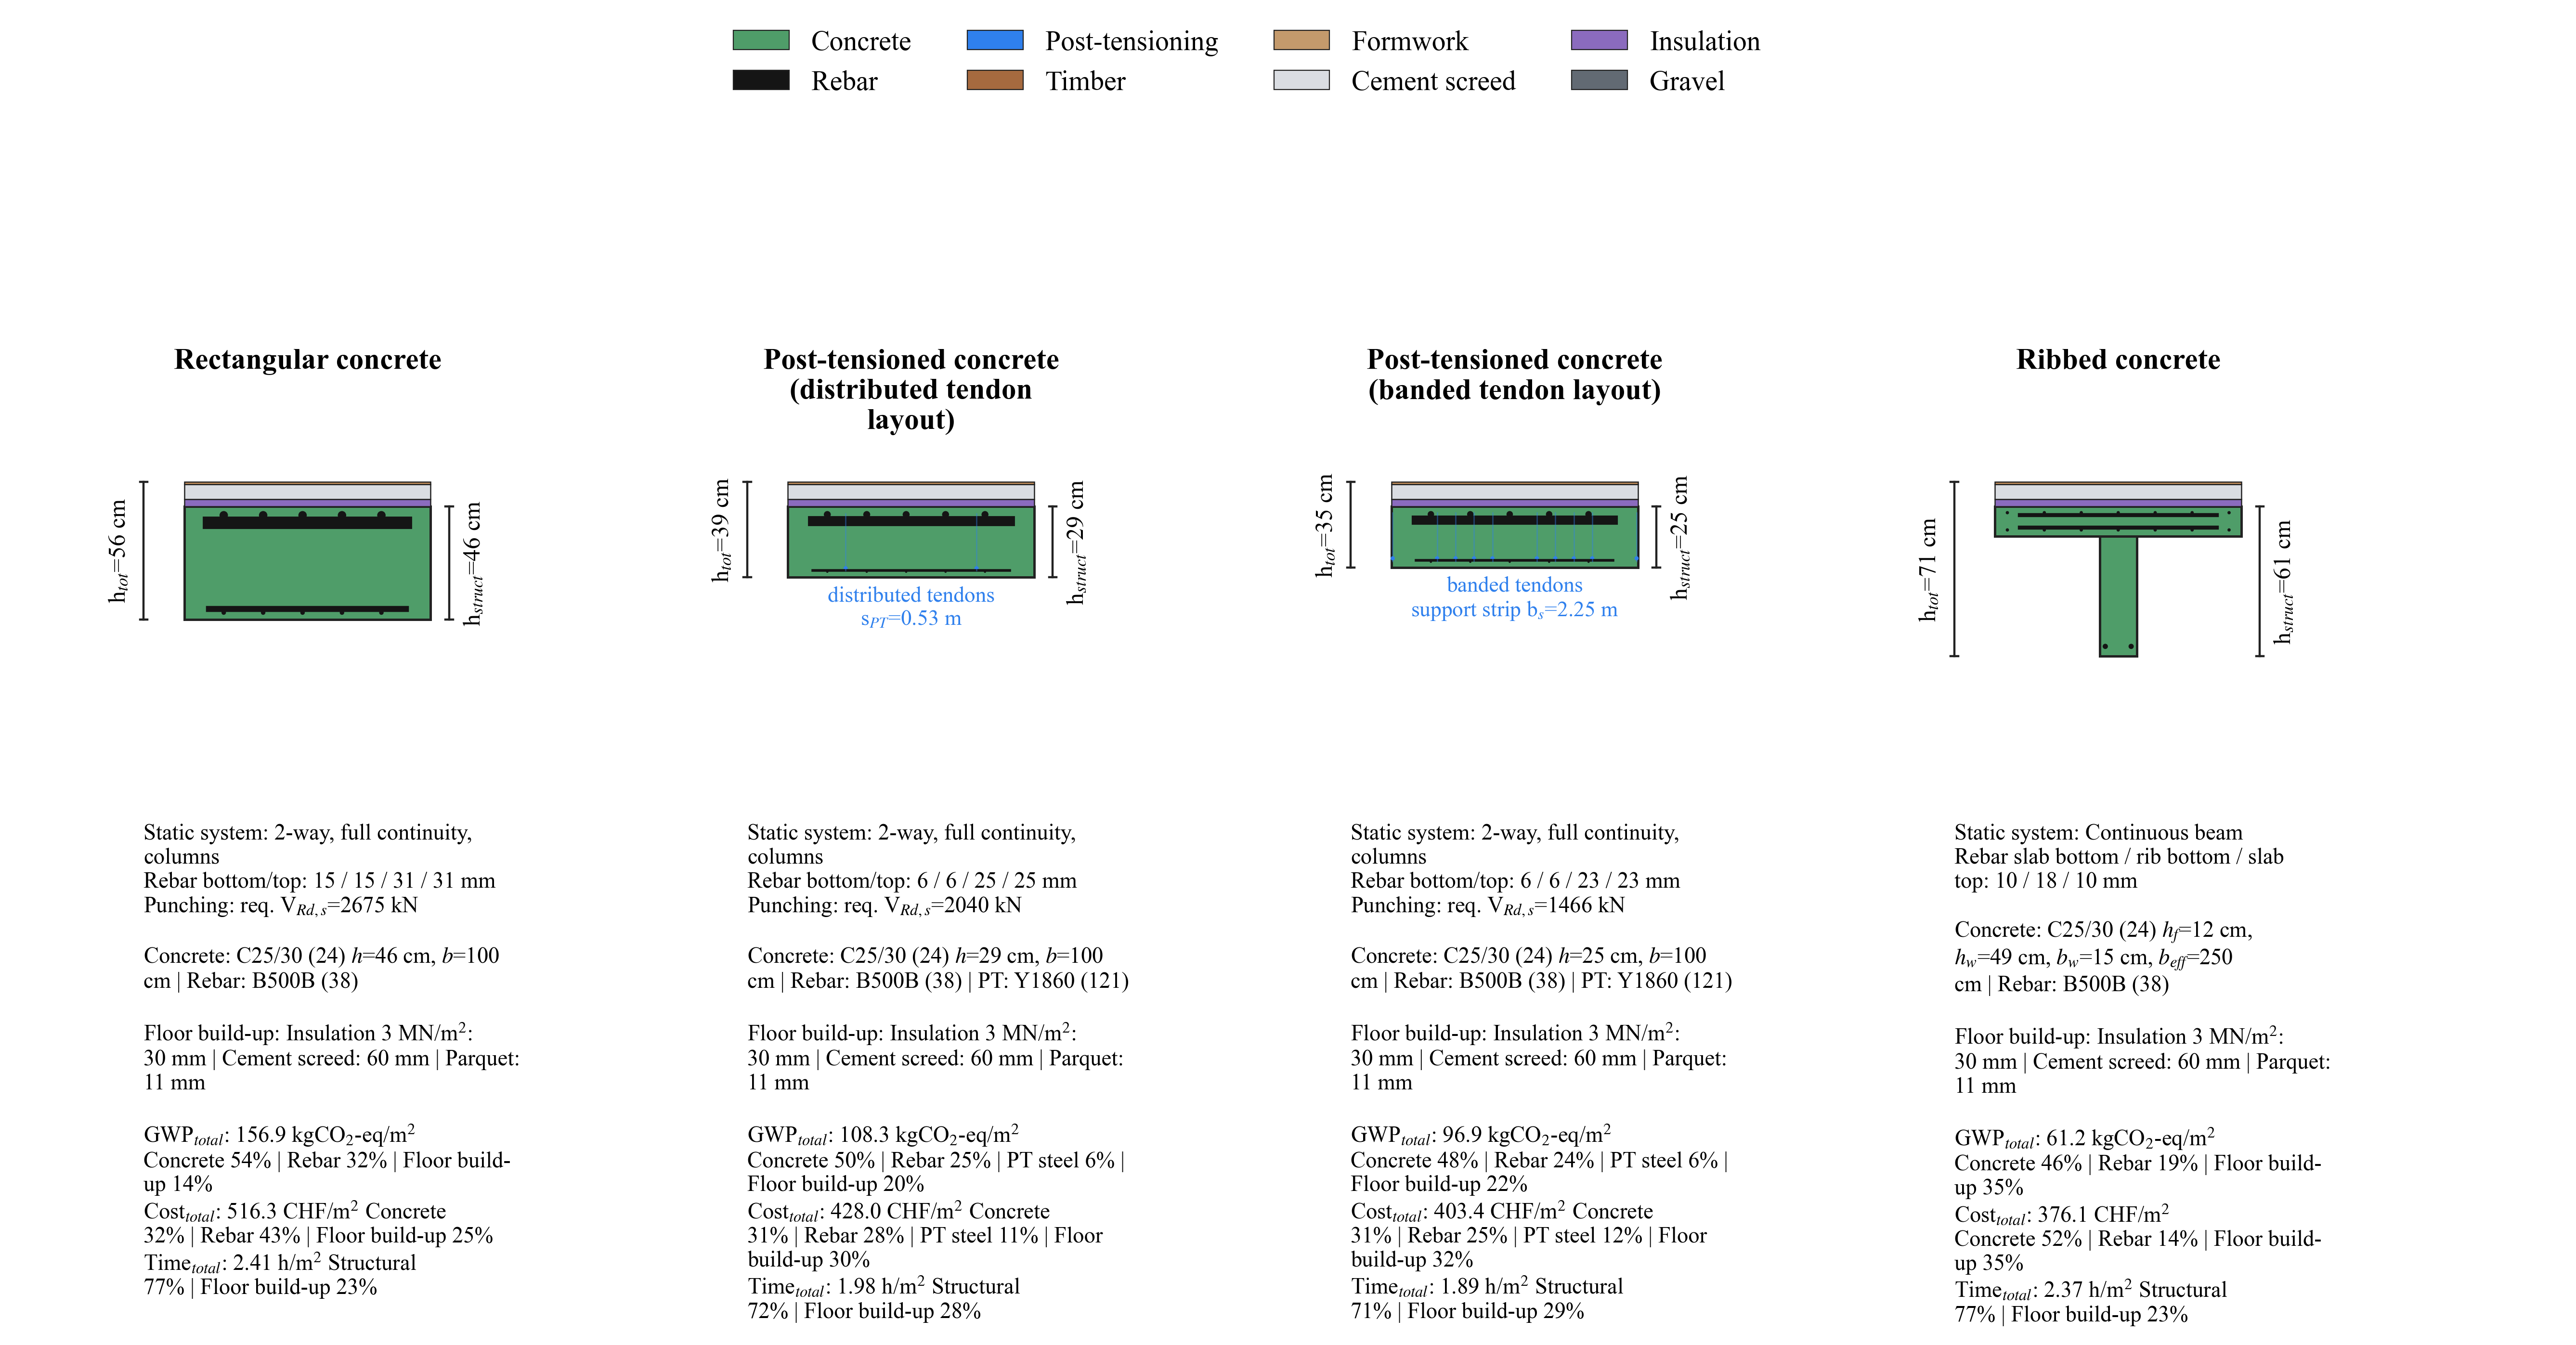
\includegraphics[width=1\textwidth]{IMAGES/final_cross_sections_office_12m.png}
    \caption{Best \(GWP_{tot}\) cross-sections for the office case at a span of \(12\,\mathrm{m}\).}
    \label{fig:final_cross_sections_office_12m}
\end{figure}

\newpage 
\subsection{Comparison of office floor systems}
The systems of the office case were compared in a similar manner to the residential case. Figure~\ref{fig:final_env_comparison_office} compares the office floor systems over the investigated span range and illustrates the variation resulting from the considered material and product datasets. Figure~\ref{fig:uq_pairwise_scores_Office} complements this comparison by the pairwise comparison. 
\begin{figure}[H]
    \centering
    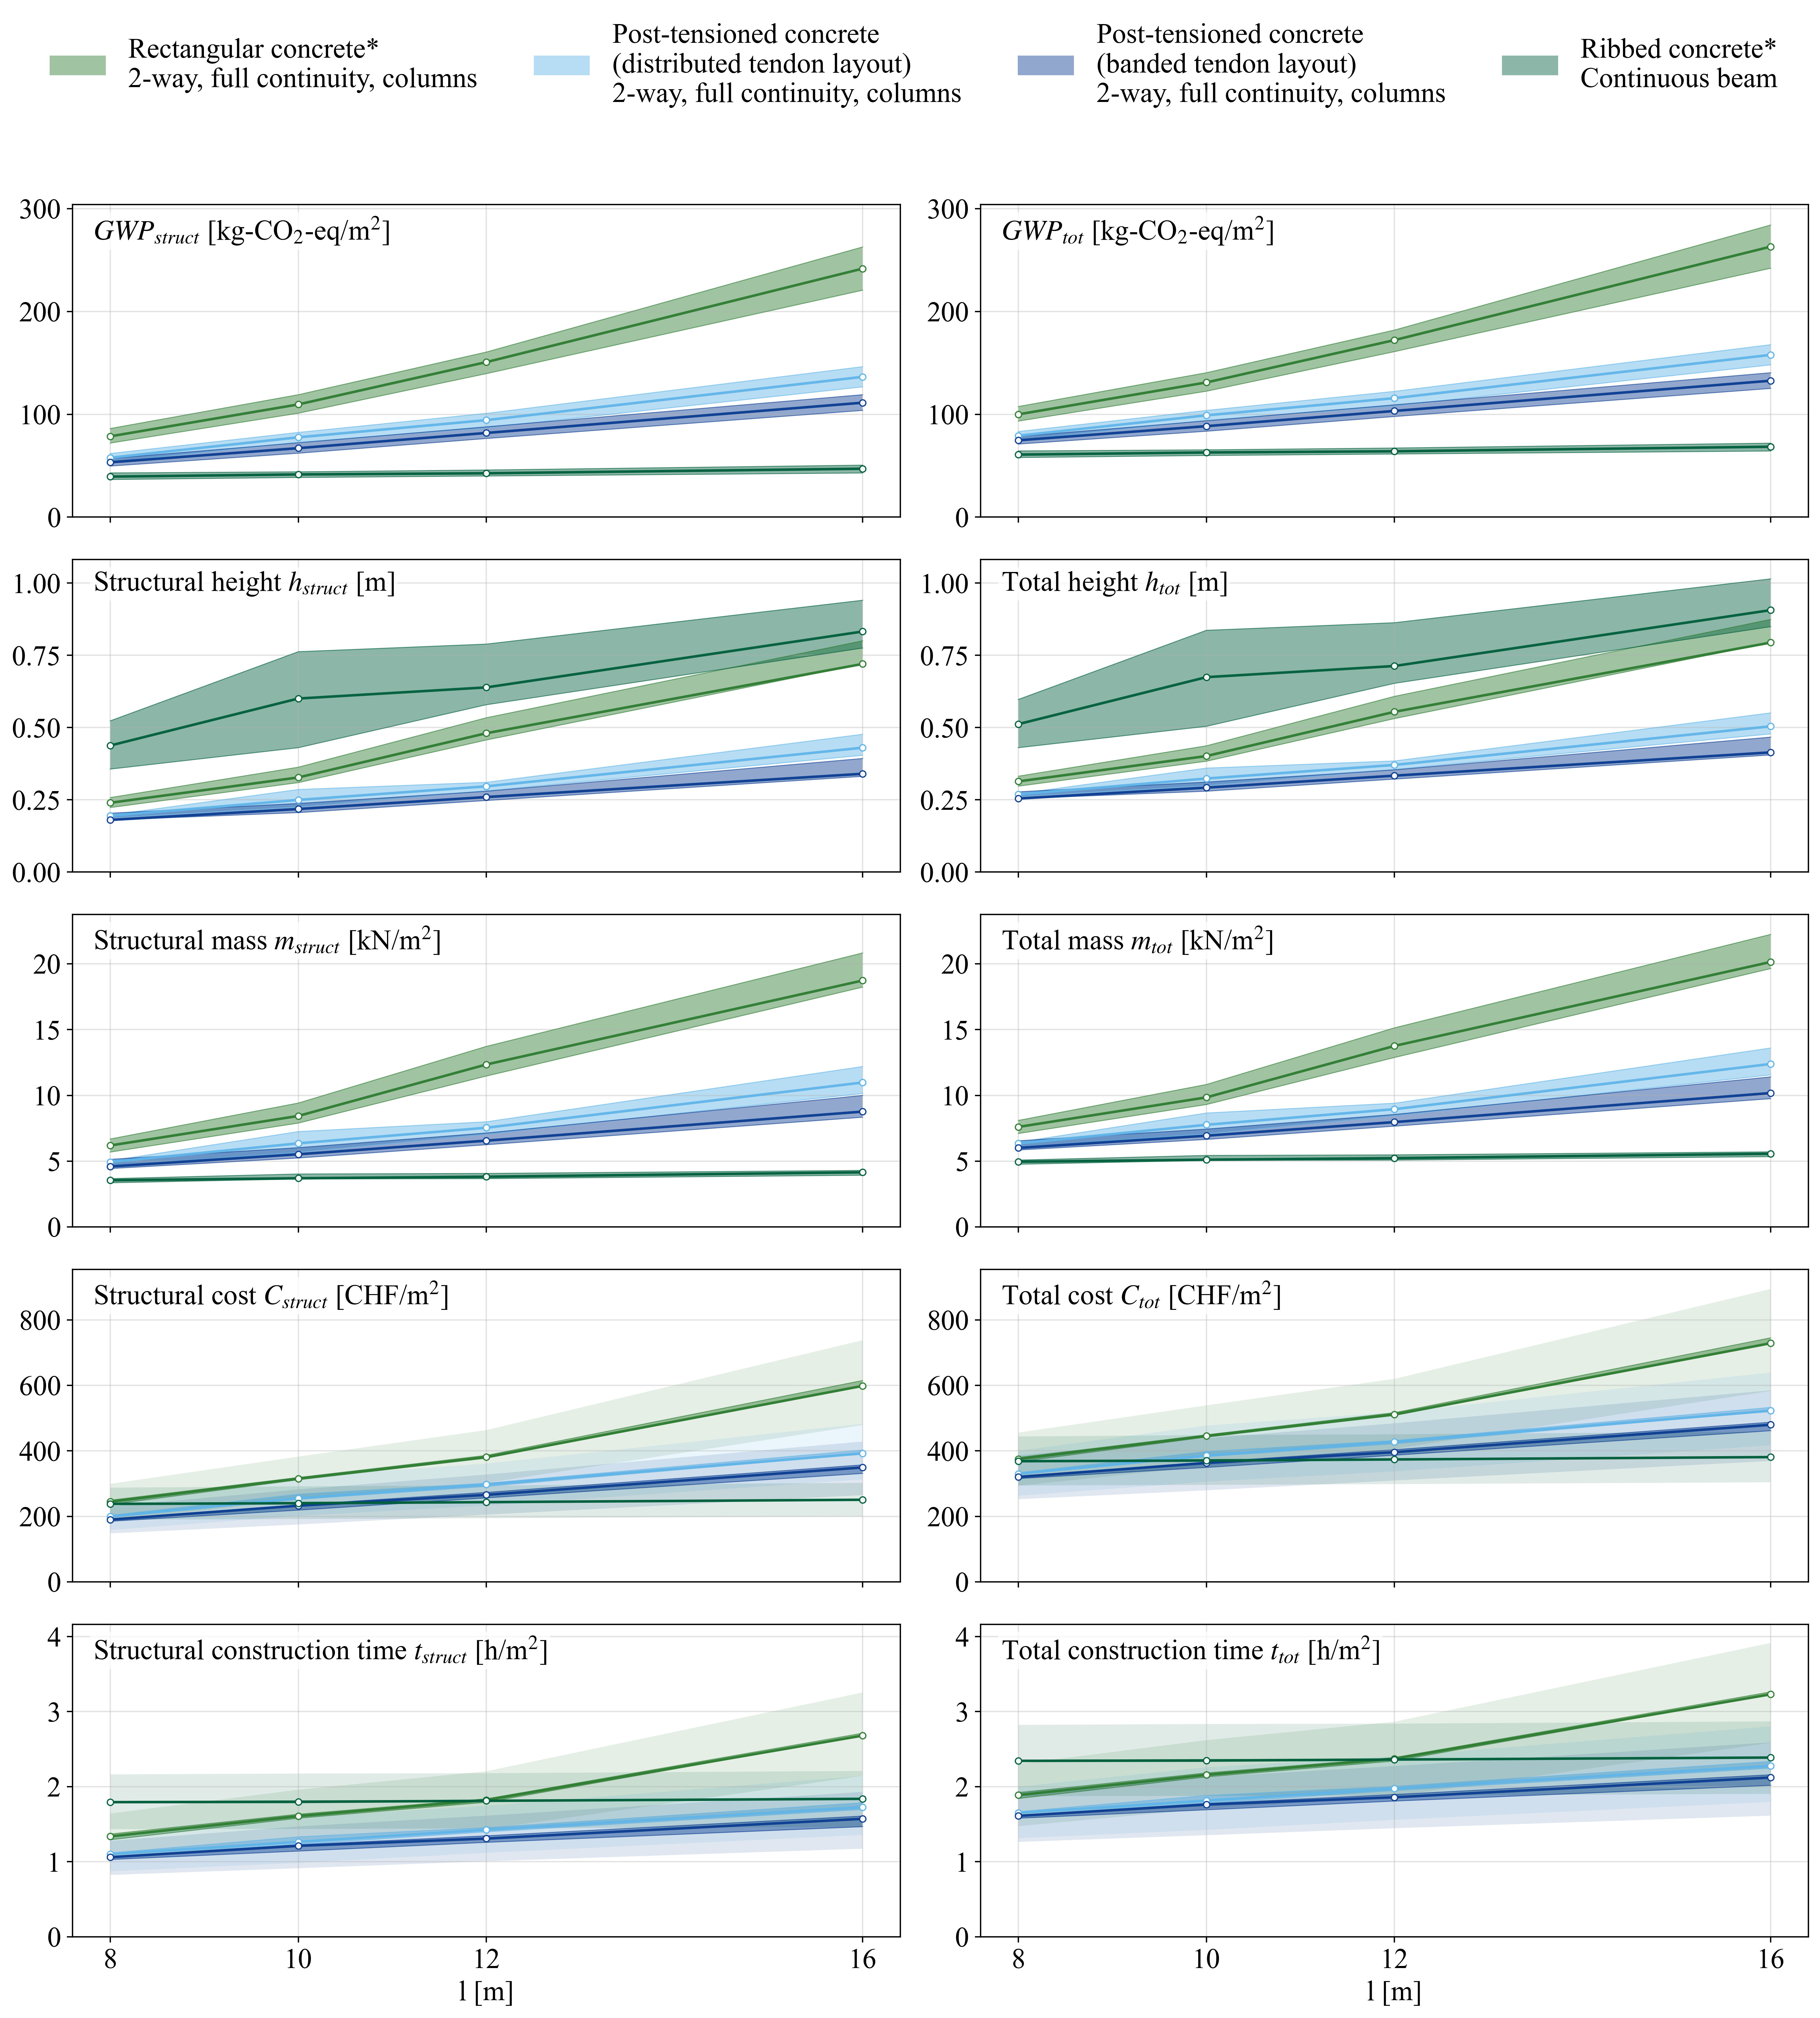
\includegraphics[width=1\textwidth]{IMAGES/final_env_comparison_office.png}
    \caption{Comparison according to sustainability assessment criteria of selected floor systems for office buildings.}
    \label{fig:final_env_comparison_office}
\end{figure}

In contrast to the residential case, only concrete-based systems are considered for the office case. Therefore, the distinction between the structural cross-section and the total floor system is less pronounced, since no comparatively heavy acoustic timber floor build-ups are required. The comparison is thus mainly governed by the structural efficiency of the concrete systems, the influence of post-tensioning, and the additional formwork demand of ribbed concrete.

\begin{figure}[H]
    \centering
    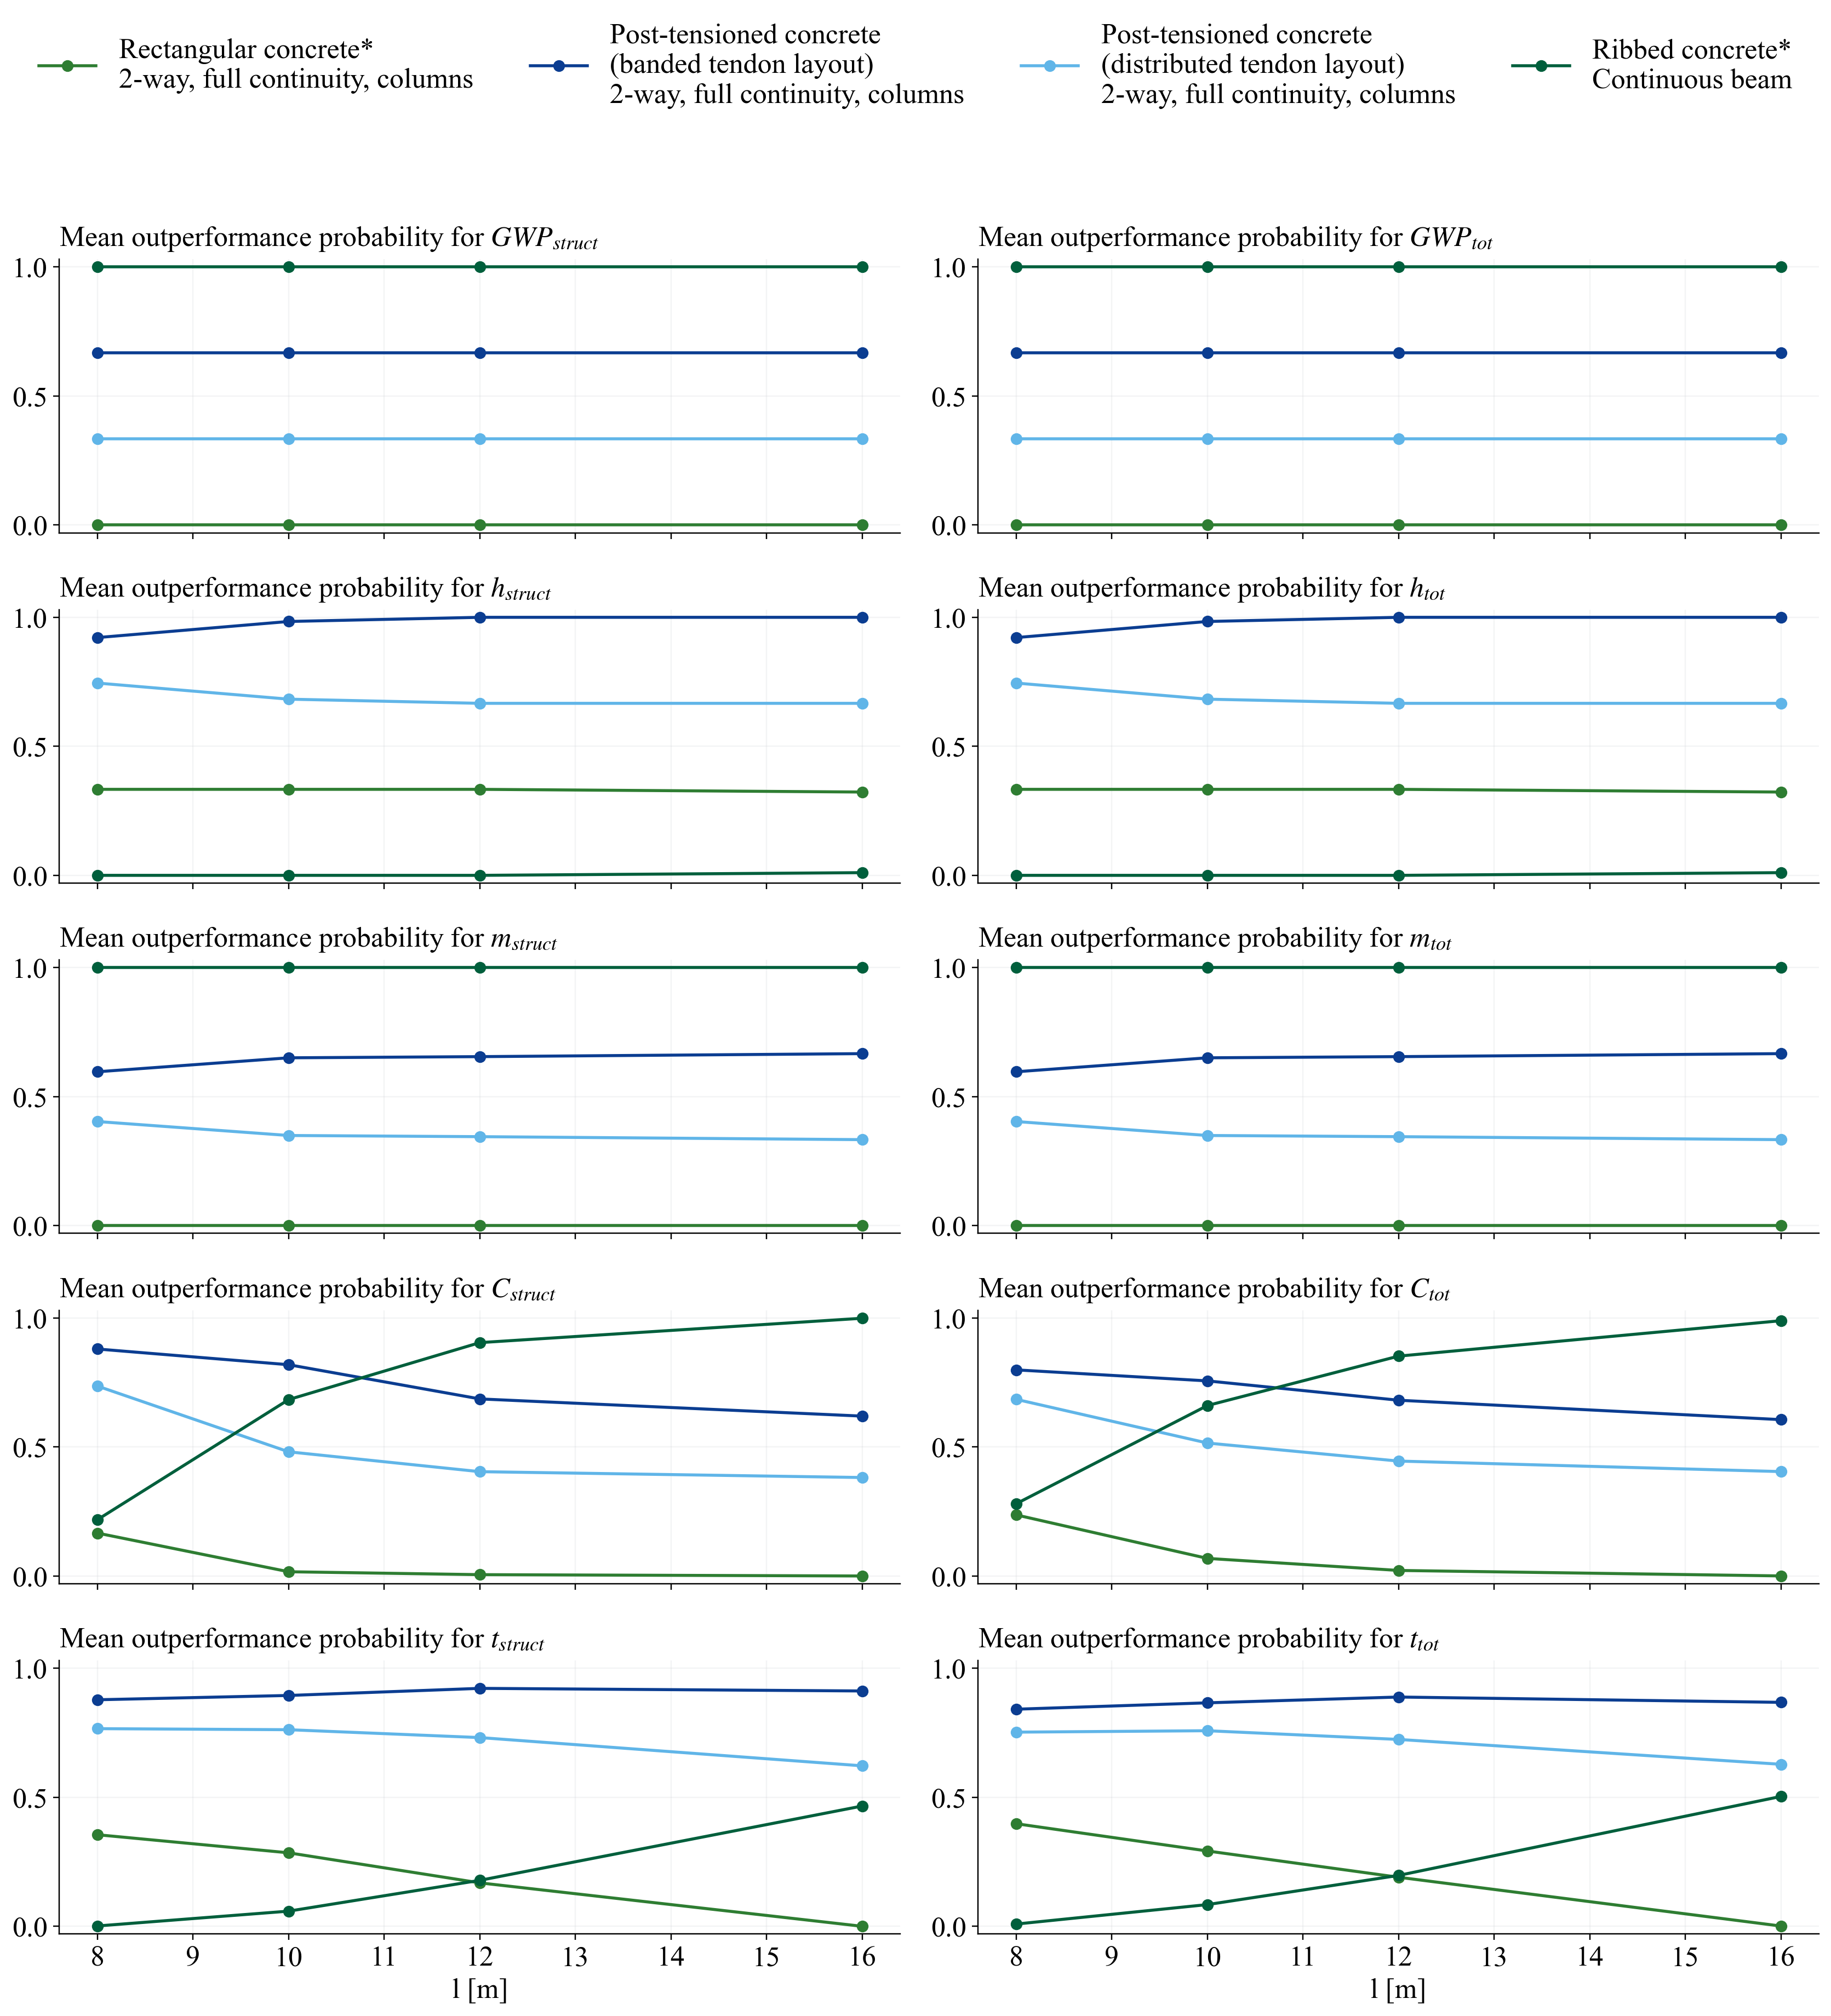
\includegraphics[width=1\textwidth]{IMAGES/uq_pairwise_scores_Office.png}
    \caption{Pairwise comparison according to sustainability assessment criteria of selected floor systems for office buildings.}
    \label{fig:uq_pairwise_scores_Office}
\end{figure}


\subsubsection{Global warming potential}

In Figure~\ref{fig:final_env_comparison_office}, ribbed concrete achieves the lowest \(GWP_{struct}\) over the investigated span range. This is also reflected in Figure~\ref{fig:uq_pairwise_scores_Office}, where ribbed concrete ranks favourably in the pairwise comparison for structural GWP. The reason is the efficient ribbed cross-section geometry, which reduces the self-weight of the cross-section while retaining sufficient bending stiffness and resistance.

Post-tensioned concrete becomes increasingly competitive with span. Compared with rectangular reinforced concrete, both post-tensioned layouts show a lower increase in \(GWP_{struct}\) over the span range. The banded tendon layout performs particularly well in the present model because the tendons are concentrated in the support strips, where the ULS checks are performed. Beneficial secondary support moments therefore reduce the governing negative support demand more effectively than in the distributed tendon layout. This effect is heavily influenced by the calculation model and must be analysed further. However, it can be hypothesised that the banded layout is a structural optimisation for post-tensioned systems and supports literature that assumes it to be a feasible post-tensioning layout \cite{PTI2023}.

Rectangular reinforced concrete shows the strongest increase in \(GWP_{struct}\) with span. This reflects the increasing slab thickness and reinforcement demand required to satisfy ULS bending. It is increasingly outperformed by post-tensioned and ribbed systems at spans above \(8\,\mathrm{m}\), aligning well with literature \cite{Rombach2010}.

\subsubsection{Height}

Figure~\ref{fig:final_env_comparison_office} shows that the post-tensioned systems achieve the lowest construction height across the investigated span range. Conventionally reinforced rectangular concrete remains competitive up to spans of \(10\,\mathrm{m}\), but then increases considerably in height, reaching values close to ribbed concrete. This is attributed to the inefficient use of material in a solid rectangular cross-section with a poor bending stiffness in relation to the self-weight.

Ribbed concrete requires a larger construction depth than the solid slab systems. Its low \(GWP_{struct}\) is therefore achieved at the cost of increased floor height. The relevance of floor height can again be illustrated using the regular building zone of the City of Zurich, where the maximum building height is limited to \(25\,\mathrm{m}\) \cite{StadtZuerich_Bauordnung_700100}.

Assuming an office room height of \(2.7\,\mathrm{m}\), the required floor depth directly affects the possible number of storeys. For a span of \(12\,\mathrm{m}\), the investigated ribbed concrete solution would allow seven storeys, whereas the post-tensioned concrete solution would allow eight storeys within the same building height. The height criterion can therefore directly influence the achievable usable floor area and should be analysed carefully.

\subsubsection{Mass}

The mass comparison follows the cross-section efficiency of the members. Ribbed concrete achieves the lowest mass as concrete is removed from structurally less effective zones of the cross-section. 

Post-tensioned concrete reduces the required concrete and reinforcement quantities compared with rectangular reinforced concrete, especially at longer spans. Therefore, it shows a more favourable mass development over the span range. Rectangular reinforced concrete becomes increasingly heavy at larger spans due to the rising demand for slab thickness and reinforcement.

Since all compared office systems require a comparable floor build-up, the differences in structural floor mass are also observed for the total cross-sections. Thus, the relevance of mass is rated higher for office buildings than for residential buildings. First, the differences between the compared systems are larger. Second, larger building envelopes are assumed for office buildings, which influence the magnitude of indirect effects on columns, foundations and lateral load-resisting systems.

\subsubsection{Construction cost}

Rectangular reinforced concrete remains economically attractive at shorter spans due to its simple geometry, established construction process, and low material cost. However, its cost increases with span as the required concrete volume and reinforcement demand increase.

Post-tensioned concrete is the most economical system for spans between approximately \(8\) and \(10.5\,\mathrm{m}\). The additional cost of tendons, anchorages, and post-tensioning operations is compensated by the reduced concrete volume and lower reinforcement demand compared with conventionally reinforced concrete. At longer spans, ribbed concrete becomes increasingly competitive because its efficient cross-section reduces material quantities. At shorter spans, however, this advantage is partly offset by the additional formwork effort caused by the ribbed geometry.

Overall, the cost performance is less pronounced than the structural GWP performance. The pairwise comparison shows that the banded post-tensioned slab has the highest total score across the investigated office span range. Ribbed concrete ranks best for \(GWP_{tot}\) and mass at all office spans and also becomes the most robust cost option from \(12\,\mathrm{m}\), but its larger construction height and longer construction time reduce its total pairwise score. The results therefore support post-tensioned concrete as the most robust overall office solution, while ribbed concrete should be selected when GWP or mass are prioritised and additional floor depth is acceptable.

\subsubsection{Construction time}

Post-tensioned concrete shows the shortest construction time across the investigated span range. The model therefore indicates that the additional process complexity of post-tensioning is offset by the reduced material demand.

Rectangular reinforced concrete shows a strong increase in construction time with span. This is mainly caused by the increasing material volume and reinforcement demand required to satisfy the structural and serviceability criteria. The heavier cross-sections at longer spans therefore directly translate into higher construction effort.

Ribbed concrete is initially penalised by the more complex formwork geometry. For spans larger than \(12\,\mathrm{m}\), the reduced material use increasingly compensates for this initial complexity, making ribbed concrete also competitive in terms of construction time.

\newpage
\section{GWP--cost correlation}
\label{sec:gwp_cost_relationship}

A conflict between GWP and construction cost is often reported in the literature \cite{Ammann2024}. In the present results, this conflict is mainly observed in the residential case, as shown in Figure~\ref{fig:scatter_gwp_total_vs_cost_total_by_case}. Based on the pairwise comparison, rectangular timber outperforms the other systems regarding \(GWP_{tot}\) at shorter spans, but it does not outperform them regarding total cost. Rectangular reinforced concrete shows the opposite tendency: it is robust regarding cost and construction height at short and intermediate spans, but it does not provide the lowest \(GWP_{tot}\). Flat TCC and ribbed TCC therefore become important compromise solutions. Flat TCC performs well when the total system is assessed across several criteria, while ribbed TCC becomes the strongest residential option at the longest investigated span.

The pairwise comparison is important because the deterministic lowest-\(GWP\) solution is not necessarily the most robust multi-criteria solution. In the residential case, rectangular timber is the clear overall pairwise winner only at the shortest investigated span. Flat TCC and rectangular reinforced concrete then alternately outperform the other systems in the intermediate range, depending on whether time and GWP or cost and height dominate the comparison. At the longest residential span, ribbed TCC outperforms the other systems in the total pairwise assessment, although post-tensioned concrete and flat TCC remain close alternatives.

The conflict between GWP and cost can therefore be tackled by separating the assessment into two steps. First, systems that are clearly dominated in the pairwise comparison should be excluded, since they do not robustly outperform the alternatives in any relevant criterion. Second, the remaining systems should be selected according to project-specific priorities. If low embodied carbon is the main objective, timber or TCC systems become preferable despite their higher modelled cost. If construction cost or floor height is the governing constraint, rectangular or post-tensioned concrete systems can be justified even when they show a higher \(GWP_{tot}\). For cases where no criterion is dominant, the pairwise comparison provides a transparent compromise by showing which system most consistently outperforms the alternatives across GWP, cost, height, mass and construction time.

The office case shows a different relationship. Since only concrete-based systems are compared, material efficiency affects both \(GWP_{tot}\) and \(Cost_{tot}\) in a similar direction. Ribbed concrete outperforms the other office systems regarding \(GWP_{tot}\) and mass across the investigated span range. It also becomes increasingly competitive regarding cost at larger spans. However, it does not achieve the best total pairwise result because its greater construction height and longer construction time reduce its overall robustness.

Accordingly, the banded post-tensioned concrete slab is the most robust office solution in the pairwise comparison. It does not show the lowest \(GWP_{tot}\), but it combines comparatively low GWP with lower construction height, shorter construction time and competitive cost. The office recommendation is therefore not based on the lowest environmental value alone, but on the system that most consistently outperforms the alternatives across the complete set of criteria.

Overall, the comparison shows that the relationship between \(GWP\) and construction cost depends strongly on the material scope of the design space. In the residential case, low-carbon solutions are not automatically low-cost solutions because timber and TCC systems are governed by different cost assumptions and construction processes. In the office case, where all systems are concrete-based, material efficiency becomes the common driver of both criteria. The conclusion is therefore not that one criterion can replace the other, but that their interaction must be interpreted separately for each building type and material family and should be evaluated with the pairwise comparison when defining application ranges.

The cost results for timber systems should be interpreted with particular caution. Their unit price is defined per cubic metre and implicitly includes fabrication and connection effort. This may overestimate the cost increase for larger timber cross-sections, because part of this effort is likely to be fixed or only weakly dependent on volume in practice. The timber cost model should therefore be validated against market data before deriving final economic recommendations. A further way to address the conflict is to include shadow carbon costs or project-specific carbon budgets in the decision process. This would make the environmental benefit of lower-GWP systems visible in economic terms and would allow designers to identify the point at which a higher construction cost is justified by the avoided emissions. Nevertheless, the observed difference between concrete and timber systems remains relevant, since a carbon price would likely have stronger leverage on concrete systems than on timber systems.

\begin{figure}[H]
    \centering
    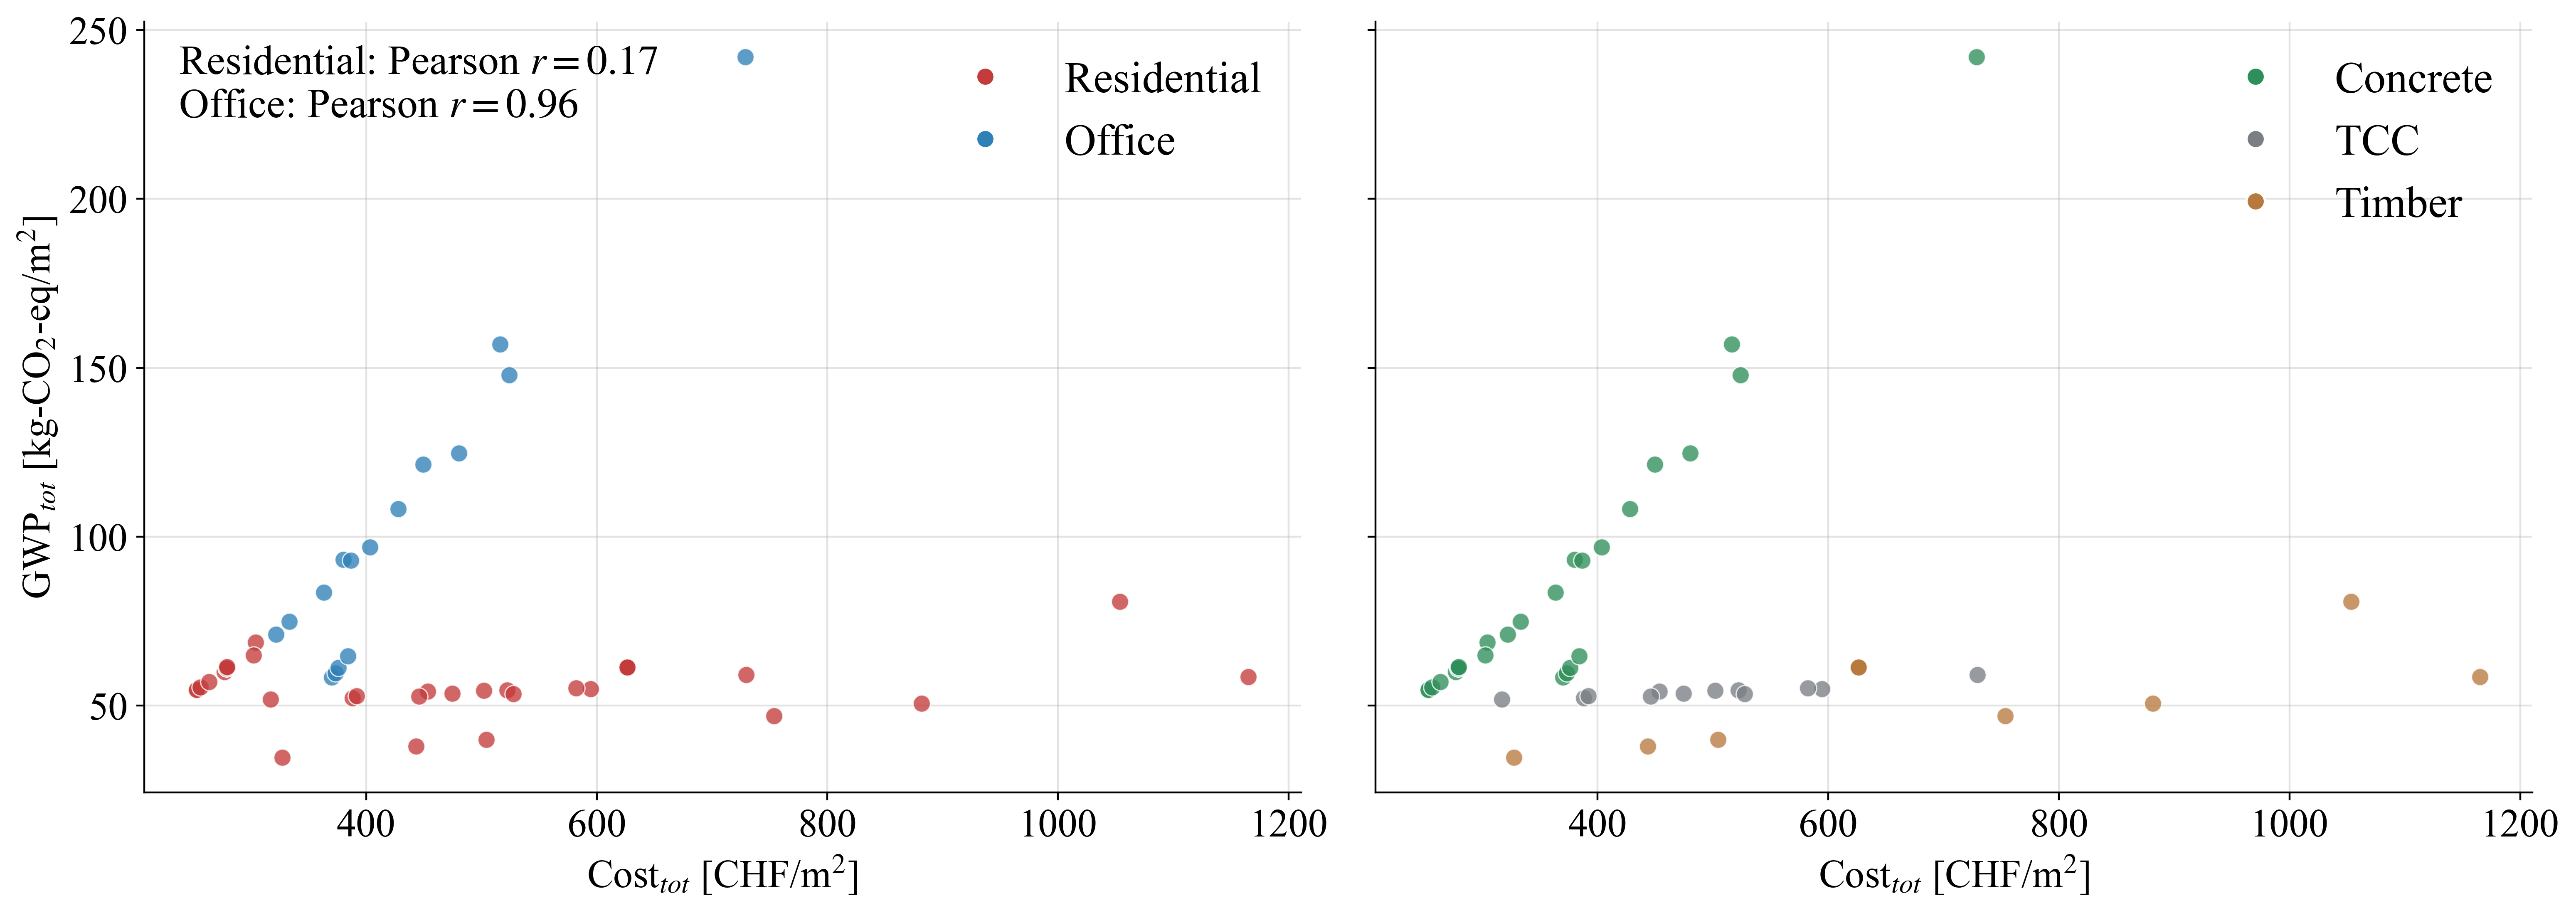
\includegraphics[width=1\textwidth]{IMAGES/scatter_gwp_total_vs_cost_total_by_case.png}
    \caption{Scatter plots between \(GWP_{tot}\) and \(Cost_{tot}\).}
    \label{fig:scatter_gwp_total_vs_cost_total_by_case}
\end{figure}
